% BtP workshop submission (CoRL 2026, "Everything Beneath the Policy"). Draft v3.2 (3 Oct 2026, with the round-2 results).
% IEEEtran conference mode; 4 pages of main text, references and appendix unlimited.
% Build: docs/btp_paper/build.sh   (tectonic; runs bibtex automatically)
\documentclass[conference]{IEEEtran}
\IEEEoverridecommandlockouts

\usepackage[T1]{fontenc}
\usepackage{amsmath,amssymb}
\usepackage{graphicx}
\usepackage{booktabs}
\usepackage{multirow}
\usepackage{array}
\usepackage{xcolor}
\usepackage{tikz}
\usetikzlibrary{arrows.meta,positioning,fit,calc}
\usepackage[hidelinks]{hyperref}
\usepackage{cite}

% ---- Draft macros (remove or empty before submission) -----------------------
% \pending{...}: a number or result that needs an experiment from the BtP plan.
% \note{...}:    an editorial note for the authors.
\newcommand{\pending}[1]{\textcolor{orange!85!black}{[\textbf{pending:} #1]}}
\newcommand{\note}[1]{\textcolor{blue!70!black}{[\textit{note:} #1]}}
% "Report:" line closing each choice (no longer used in the main text; Table II carries the items).
\newcommand{\report}[1]{\textbf{Report:} #1}

% ---- Paper macros -------------------------------------------------------------
\definecolor{pitc}{RGB}{213,94,0}   % pitfalls (vermillion)
\definecolor{forkc}{RGB}{0,114,178} % forks (blue)
\newcommand{\dy}{\textit{dy}}
\newcommand{\dx}{\textit{dx}}
\newcommand{\dz}{\textit{dz}}
\newcommand{\rowid}[1]{\texttt{#1}}
\newcommand{\pit}{\textcolor{pitc}{\textbf{P}}}
\newcommand{\frk}{\textcolor{forkc}{\textbf{F}}}
\newcommand{\head}[1]{\textit{#1}\hspace{0.4em}}
\newcommand{\anon}{[anonymous companion submission]}
\newcolumntype{L}[1]{>{\raggedright\arraybackslash}p{#1}}

\begin{document}

\title{Same Outputs, Opposite Verdicts: Pitfalls and Forks Beneath a VLA Language Evaluation%
\thanks{A companion paper on the behaviour itself is under review at another CoRL 2026 workshop; this paper concerns its measurement.}}
\author{\IEEEauthorblockN{Anonymous Authors}\IEEEauthorblockA{Paper under double-blind review}}
\maketitle

\begin{abstract}
Holding one model (OpenVLA-7B) and 340 twin scenes fixed, we vary one evaluation choice at a time. On identical outputs, naive scoring of mirrored scenes points the word effect toward the named twin (21 of 25 splits) and correct scoring points it away (4 of 25), and the wrong axis makes the stimuli seem to fail. A direction-blind contrast scores two instructions naming the same twin as high as ``left'' versus ``right''. We separate pitfalls, conventions with a right answer that need a reported check, from forks, choices without one that need a specification curve. Two conclusions survive every one-at-a-time variation: the model does not reliably select the named twin, and its two instructions mostly move the same way. Pre-processing and 4-bit inference change most actions but no wording's direction. Fragile: the residual word effect's direction and the direction-blind contrast's significance. A pre-declared specification curve over 256 analyses agrees: wording explains 42\% of the word effect's variance, and no analysis shows reliable selection. We map a reporting card onto the workshop checklist's announced categories.
\end{abstract}

% =============================================================================
\section{Introduction}
\label{sec:intro}

Robot-learning results rest on choices beneath the policy~\cite{park2026everything}. We audit those that sit between a policy's output and an evaluation's verdict, in one model organism: a probe of whether OpenVLA-7B~\cite{kim2024openvla} uses ``left'' and ``right'' to choose between an object and its mirrored copy (twins) in real BridgeData~V2 frames~\cite{walke2023bridgedata}. For token-based policies such as OpenVLA, the readout from logits to commands is part of the action space, and an evaluation's conventions are part of the substrate.

Choices that leave every model output unchanged can reverse the verdict (Fig.~\ref{fig:pipeline}; bf16 unless marked). In \emph{opposite} scenes one twin lies on each side of the gripper; a \emph{split} is a scene in which the two instructions move the arm apart. On mirrored images, correct scoring finds the residual word effect pointing away from the named twin (4 of 25 splits toward it, $p=.0009$); negating the expected direction instead, as mirror augmentation negates actions, turns the same outputs into 21 of 25. A direction-blind contrast (do instructions split more often in opposite than in same-side scenes?) scores two instructions naming the same twin, ``grab'' and ``take the \{noun\} on the left'', at $+11.7$ points ($p=.012$), as high as ``left'' versus ``right''. Read on the wrong action axis, the stimuli seem not to work ($p=1.0$). Other choices change the question: the wording sets the word effect's direction, and 4-bit inference changes 58--67\% of lateral tokens but no wording's direction.

\emph{Pitfalls} are conventions with a right answer, such as the sign of the lateral axis or the scoring of mirrored scenes; set wrongly, they can silently reverse or erase a verdict, so papers should report the convention and the check that verified it. \emph{Forks} have no single right answer. Some change the question, the estimand~\cite{lundberg2021what}: the executed or the expected action, one phrasing or a word across phrasings. Others, such as the decision threshold, are interchangeable ways to answer one question. Forks call for a specification curve, a factorial ablation over analysis choices plotted in sorted order~\cite{simonsohn2020specification}. We tag each choice by whether it changes the \emph{direction}, \emph{strength} or \emph{scope} (the scenes or conditions covered) of a claim, and keep \emph{selection} (are both instructions correct?) apart from \emph{direction} (which way does the word push when the actions split?).

In LLM evaluation, prompt format, readout and quantisation change answers~\cite{sclar2024quantifying,wang2024answer,dutta2024accuracy}; undocumented pipeline conventions move VLA closed-loop success~\cite{choi2026vlaeval,islam2026deployment,xu2026vlaquantbench}, and closed-loop instruments can certify absent language following~\cite{kirouane2026measuring}. Unlike these audits, we study a language verdict within one model. STAGE~\cite{jin2026stage} reads OpenVLA's single-step action under instruction swaps and already shows that direction-blind and direction-aware scores differ; we add twins with same-side controls on real frames and readouts of the action-token distribution. To our knowledge, as of early October 2026, this is the first audit of the measurement layer beneath a VLA language verdict and the first specification-curve analysis of a robot-learning evaluation (pre-declared; Sec.~\ref{sec:survives}).

We contribute (i)~a pitfall audit (Sec.~\ref{sec:pitfalls}); (ii)~a fork analysis and a pre-declared specification curve faceted by estimand (Secs.~\ref{sec:forks}--\ref{sec:survives}); (iii)~a checkable reporting card (Sec.~\ref{sec:card}); (iv)~the probe, stimuli and outputs, released at an anonymous URL.

% ---- Figure 1 -----------------------------------------------------------------
\begin{figure*}[t]
\centering
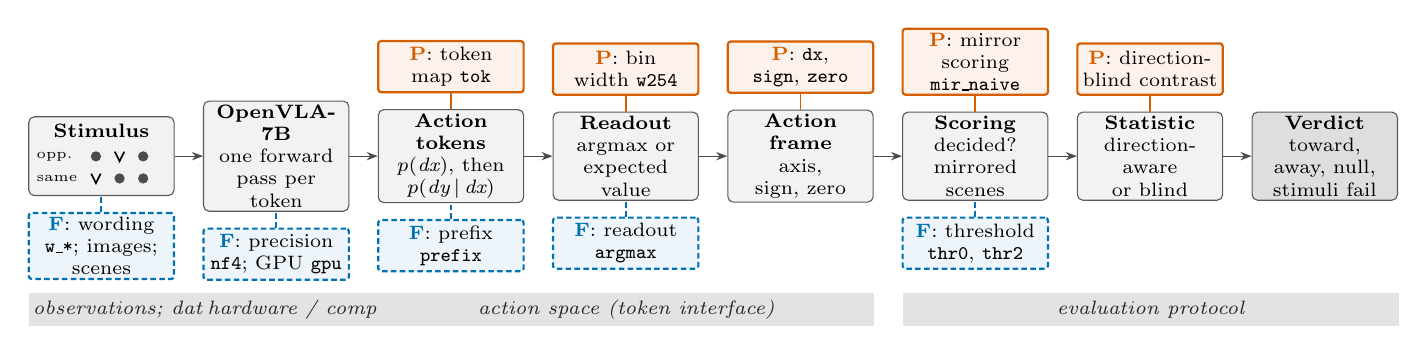
\begin{tikzpicture}[
  font=\scriptsize,
  >={Stealth[length=4pt]},
  stage/.style={draw=black!65, rounded corners=2pt, fill=black!5, minimum height=10mm,
                text width=17.4mm, align=center, inner sep=1.5pt},
  pit/.style={draw=pitc, line width=0.8pt, fill=pitc!8, text width=17.4mm, align=center,
              inner sep=1.5pt, rounded corners=1pt, minimum height=6.5mm},
  frk/.style={draw=forkc, line width=0.8pt, dash pattern=on 2pt off 1.2pt, fill=forkc!7,
              text width=17.4mm, align=center, inner sep=1.5pt, rounded corners=1pt, minimum height=6.5mm},
  lay/.style={fill=black!11, text=black!85, align=center, inner sep=1.5pt, minimum height=4.2mm,
              font=\scriptsize\itshape},
  twin/.style={circle, fill=black!70, inner sep=0pt, minimum size=1.3mm},
]
\node[stage] (s1) {\textbf{Stimulus}\\ \strut\\ \strut};
% stimulus logic: twins (dots) and gripper (V), opposite and same-side layouts
\foreach \yy/\lab/\g/\ta/\tb in {5.1/opp./11.6/8.6/14.6, 7.9/same/8.6/11.6/14.6}{
  \node[font=\tiny, anchor=west, inner sep=0pt] at ($(s1.north west)+(1.0mm,-\yy mm)$) {\lab};
  \node[twin] at ($(s1.north west)+(\ta mm,-\yy mm)$) {};
  \node[twin] at ($(s1.north west)+(\tb mm,-\yy mm)$) {};
  \draw[line width=0.6pt] ($(s1.north west)+(\g mm-0.6mm,-\yy mm+0.6mm)$) -- ($(s1.north west)+(\g mm,-\yy mm-0.6mm)$) -- ($(s1.north west)+(\g mm+0.6mm,-\yy mm+0.6mm)$);
}
\node[stage, right=3.6mm of s1] (s2) {\textbf{OpenVLA-7B}\\ one forward pass per token};
\node[stage, right=3.6mm of s2] (s3) {\textbf{Action tokens}\\ $p(\dx)$, then $p(\dy\,|\,\dx)$};
\node[stage, right=3.6mm of s3] (s4) {\textbf{Readout}\\ argmax or expected value};
\node[stage, right=3.6mm of s4] (s5) {\textbf{Action frame}\\ axis, sign, zero};
\node[stage, right=3.6mm of s5] (s6) {\textbf{Scoring}\\ decided?\ mirrored scenes};
\node[stage, right=3.6mm of s6] (s7) {\textbf{Statistic}\\ direction-aware or blind};
\node[stage, right=3.6mm of s7, fill=black!13] (s8) {\textbf{Verdict}\\ toward, away, null, stimuli fail};
\foreach \a/\b in {s1/s2,s2/s3,s3/s4,s4/s5,s5/s6,s6/s7,s7/s8} \draw[->, black!70] (\a) -- (\b);
% pitfalls (above)
\node[pit, above=2mm of s3] (p3) {\pit: token map \rowid{tok}};
\node[pit, above=2mm of s4] (p4) {\pit: bin width \rowid{w254}};
\node[pit, above=2mm of s5] (p5) {\pit: \rowid{dx}, \rowid{sign}, \rowid{zero}};
\node[pit, above=2mm of s6] (p6) {\pit: mirror scoring \rowid{mir\_naive}};
\node[pit, above=2mm of s7] (p7) {\pit: direction-blind contrast};
\foreach \n in {3,4,5,6,7} \draw[pitc, line width=0.7pt] (p\n) -- (s\n);
% forks (below)
\node[frk, below=2mm of s1] (f1) {\frk: wording \rowid{w\_*}; images; scenes};
\node[frk, below=2mm of s2] (f2) {\frk: precision \rowid{nf4}; GPU \rowid{gpu}};
\node[frk, below=2mm of s3] (f3) {\frk: prefix \rowid{prefix}};
\node[frk, below=2mm of s4] (f4) {\frk: readout \rowid{argmax}};
\node[frk, below=2mm of s6] (f6) {\frk: threshold \rowid{thr0}, \rowid{thr2}};
\foreach \n in {1,2,3,4,6} \draw[forkc, line width=0.7pt, dash pattern=on 2pt off 1.2pt] (f\n) -- (s\n);
% workshop layers (band)
\coordinate (yb) at ($(f1.south)+(0,-1.6mm)$);
\path let \p1=(s1.west), \p2=(s1.east), \p3=(yb) in node[lay, minimum width=\x2-\x1, anchor=north west] at (\x1,\y3) {observations; data};
\path let \p1=(s2.west), \p2=(s2.east), \p3=(yb) in node[lay, minimum width=\x2-\x1, anchor=north west] at (\x1,\y3) {hardware / compute};
\path let \p1=(s3.west), \p2=(s5.east), \p3=(yb) in node[lay, minimum width=\x2-\x1, anchor=north west] at (\x1,\y3) {action space (token interface)};
\path let \p1=(s6.west), \p2=(s8.east), \p3=(yb) in node[lay, minimum width=\x2-\x1, anchor=north west] at (\x1,\y3) {evaluation protocol};
\end{tikzpicture}
\caption{The measurement pipeline, with the workshop's substrate layers below and the twin layouts in the first box (dots: twins; V: gripper). Pitfalls (\textcolor{pitc}{\textbf{P}}, solid; conventions with a right answer) sit above the stage they affect, forks (\textcolor{forkc}{\textbf{F}}, dashed; choices without one) below; labels are rows of Tables~\ref{tab:oat} and~\ref{tab:oatfull}.}
\label{fig:pipeline}
\end{figure*}

% =============================================================================
\section{The probe as a model organism}
\label{sec:probe}

\head{Model and units.}OpenVLA-7B emits one token per action dimension, autoregressively (\dx\ before \dy)~\cite{kim2025finetuning}; greedy decoding is the default in its released code. We read the lateral component \dy\ of the first action. One bin, the grid step, is $3.2\times10^{-4}$ in Bridge's action units, about 0.3\,mm per 0.2-s control step~\cite{walke2023bridgedata} if, as the magnitudes indicate, the units are metres. The median first lateral command is 4.3 bins, and a scene's two instructions differ by a median of 2.4 bins (two paraphrases: 1.4), so the residual word effects below are fractions of a bin.

\head{Stimuli.}Each scene is a 640$\times$480 Bridge frame~\cite{oneill2024open} in which an object's own pixels are cut out, mirrored and pasted beside it, so that the twins lie on opposite sides of the gripper or both on one side (App.~\ref{app:stimuli}). The instruction names one twin: ``pick up the \{noun\} on the left'' (or right); image-left/right refer to the camera image. Opposite scenes separate grounding from a layout prior: grounded instructions split, each toward its own twin. Same-side scenes separate grounding from a word-to-direction shortcut: grounded instructions move the same way, whereas a shortcut would split them. After blind screening and hand labelling, 340 scenes from 191 base frames remain (93 both-left, 151 opposite, 96 both-right).

\head{Reference analysis.}Each choice starts at a reference value (Table~\ref{tab:oat}, row \rowid{ref}): \dy\ with image-right negative and physical zero; the expected value over all 256 action tokens, edge token folded, which has no ties (argmax ties in 30\% of pairs); decided if $|\dy|\geq$ one bin, a deadband; bf16 on an NVIDIA GH200; original wording and images; all scenes; correct mirror scoring. \emph{Headline} rates: same-sign, both-correct and image-right shares by layout. The signed left$-$right median over all pairs is positive toward the named twin's side, as grounding predicts, but a word-to-direction shortcut predicts it too. Its $p$-values in the text come from sign-flip tests by base frame (App.~\ref{app:defs}). 4-bit logs from an NVIDIA A100, with only a 255-token readout, replicate the reference's headline rates.

\head{Behaviour.}In the reference run both instructions move the same way in 81.2\% of opposite scenes and both are correct in 6.2\% (7/112): no selection. The action follows the layout, image-right in 44\%, 71\% and 99\% of both-left, opposite and both-right scenes. A companion paper studies this behaviour \anon. As a positive control, moving only the paste shifts the term-free (no lateral word) \dy\ action toward it by a median of 1.4 bins, 32\% of the median command (73.2\% of 149 frames, $p=5.6\times10^{-7}$).

% ---- Table 1 --------------------------------------------------------------------
\begin{table*}[t]
\centering
\scriptsize
\setlength{\tabcolsep}{2.2pt}
\caption{One-at-a-time sensitivity: each row changes one choice from the reference (Sec.~\ref{sec:probe}). Rates (\%) over decided opposite scenes; image-right by layout (both-left/opposite/both-right). Changes: \emph{direction}, a directional statistic changes sign; \emph{strength}, size or significance changes without. Direction-blind: contrast (McNemar); direction-aware: splits (binomial), signed median (Wilcoxon; positive toward the named twin's side). $p$ uncorrected. Verdict: sign of the signed effect at $p<.05$; $^\ddagger$survives Holm over 48 tests (App.~\ref{app:oat}). $^\ast$Image-right $=$ negative \dx. $^\dagger$30\% ties, rank-biserial $-0.16$. $^\S$A100, bf16: compare with the row below it, not with the reference (\rowid{prefix}: own \dx; \rowid{screen}: approved composites, both scored by recorded layout).}
\label{tab:oat}
\begin{tabular}{@{}l c l l r c r r r l@{}}
\toprule
Row & Kind & Changes & Choice changed & Both correct & Image-right & Contrast, pts ($p$) & Splits right way ($p$) & Signed, bins ($p$) & Verdict\\
\midrule
\rowid{ref} & -- & -- & Reference analysis & 6.2 & 44/71/99 & $+10.7$ (.039) & 7/21 (.189) & $-0.15$ (.011) & away\\
\midrule
\rowid{dx} & \pit & strength & Axis: \dx\ instead of \dy$^\ast$ & 4.2 & 82/82/78 & $-1.8$ (.774) & 6/12 (1.000) & $+0.09$ (.051) & null; flat layout\\
\rowid{sign} & \pit & direction & Sign: image-right $=$ positive \dy & 12.5 & 56/29/1 & $+10.7$ (.039) & 14/21 (.189) & $+0.15$ (.011) & toward\\
\rowid{zero} & \pit & strength & Zero: normalised zero ($-1.3$ bins) & 6.2 & 24/57/99 & $+12.0$ (.012) & 7/21 (.189) & $-0.15$ (.011) & away\\
\rowid{mir\_naive} & \pit & direction & Mirror scoring: negated, not swapped & 18.3 & 39/79/86 & $+1.3$ (1.000) & 21/25 (.00091) & $+0.49$ (.00077) & toward$^\ddagger$\\
\midrule
\rowid{argmax} & \frk & strength & Readout: argmax token & 8.3 & 45/72/98 & $+6.9$ (.227) & 9/20 (.824) & $0.00$ (.038)$^\dagger$ & away\\
\rowid{thr0} & \frk & strength & Threshold: any nonzero action & 10.6 & 49/68/97 & $+1.6$ (.864) & 16/35 (.736) & $-0.15$ (.011) & away\\
\rowid{thr2} & \frk & strength & Threshold: 2 bins & 6.7 & 37/73/99 & $+14.0$ (.008) & 6/17 (.332) & $-0.15$ (.011) & away\\
\rowid{nf4} & \frk & strength & Precision: 4-bit NF4 (same GH200) & 6.0 & 39/70/94 & $+4.1$ (.549) & 7/19 (.359) & $-0.03$ (.215) & null\\
\rowid{gpu} & \frk & none & GPU: A100, 4-bit, 255-token readout & 5.1 & 38/71/94 & $+4.1$ (.549) & 6/19 (.167) & $-0.02$ (.485) & null\\
 & & & \quad vs GH200, same settings & 6.1 & 39/71/94 & $+4.1$ (.549) & 7/19 (.359) & $-0.03$ (.240) & null\\
\rowid{prefix} & \frk & strength & Prefix: \dx\ fixed at the term-free token$^\S$ & 4.2 & 42/74/98 & $+4.7$ (.29) & 5/12 (.77) & $-0.02$ (.010) & away\\
 & & & \quad vs reference settings on an A100 & 7.1 & 42/71/99 & $+10.5$ (.008) & 8/20 (.50) & $-0.06$ (.070) & null\\
\rowid{mir} & \frk & strength & Images: mirrored, correctly scored & 3.5 & 39/79/86 & $+1.3$ (1.000) & 4/25 (.00091) & $-0.49$ (.00077) & away$^\ddagger$\\
\rowid{w\_prenominal} & \frk & direction & Wording: ``pick up the left \{noun\}'' & 18.7 & 34/69/99 & $+15.7$ (.013) & 20/26 (.009) & $+0.35$ (.00075) & toward$^\ddagger$\\
\rowid{w\_object} & \frk & direction & Wording: ``\dots\ the object on the left'' & 20.4 & 48/62/82 & $+3.7$ (.607) & 23/31 (.011) & $+0.25$ (.010) & toward\\
\rowid{w\_table\_side} & \frk & strength & Wording: ``\dots\ left side of the table'' & 2.7 & 49/73/95 & $+9.6$ (.039) & 3/24 (.00028) & $-0.48$ (1.1e$-$5) & away$^\ddagger$\\
\rowid{sub\_det} & \frk & strength & Scenes: detected gripper (199 of 340) & 4.5 & 50/73/100 & $+6.1$ (.375) & 3/11 (.227) & $-0.37$ (.002) & away\\
\rowid{screen} & \frk & strength & Scenes: 824 screened-out composites$^\S$ & 8.1 & 40/63/83 & $+2.0$ (.711) & 22/54 (.220) & $-0.14$ (.001) & away\\
 & & & \quad vs the 820 approved composites & 5.4 & 47/72/88 & $+6.4$ (.064) & 17/54 (.009) & $-0.10$ (.0005) & away\\
\bottomrule
\end{tabular}
\end{table*}

% =============================================================================
\section{Pitfalls: conventions with a right answer}
\label{sec:pitfalls}

A pitfall's wrong branch is not a reasonable specification~\cite{simonsohn2020specification}, so we audit it rather than vary it (rows \pit\ in Table~\ref{tab:oat}); Table~\ref{tab:card} names each check.

\head{Mirror scoring (observations; direction).}The rule is to score each instruction against the twin it names in the image the model sees: after a horizontal flip, ``the mug on the left'' still asks for image-left motion but names the other twin, which is why grounding codebases swap the words when they flip~\cite{kamath2021mdetr,deng2021transvg}. Mirror augmentation instead negates the demonstrated lateral action~\cite{zhuang2025mirrorduo}; negating the expected direction in the same way, without changing which twin each word names, exchanges the splits that go the right way with those that go the wrong way. On the bf16 mirrored outputs this turns 4 of 25 right-way splits into 21 of 25 (both $p=.0009$, surviving Holm) and the signed effect from $-0.49$ into $+0.49$ bins. A significantly reversed result is scored as significant grounding. Mirrored robot images are out of distribution~\cite{zhuang2025mirrorduo}, so we treat them as an exploratory replication.

\head{The direction-blind statistic (evaluation protocol; direction).}Sign agreement between a scene's two actions is unchanged when every ``left'' label is swapped with ``right'', which turns grounded behaviour into its reverse. The same-side minus opposite contrast therefore cannot separate the two at any sample size and can call backwards behaviour significant, akin to a sign (Type~S) error~\cite{gelman2014beyond}: in the 4-bit GH200 run, ``\dots\ on the left side of the table'' gives $+14.8$ points ($p=.004$; Holm-adjusted .017) while its signed effect is reversed ($-0.53$ bins, $p<10^{-4}$). Nor is it specific to the spatial word: two instructions that name the same twin give $+11.7$ points (McNemar $p=.012$) in the reference run, as much as ``left'' versus ``right'' ($+10.7$, $p=.039$ uncorrected). On the A100 runs (bf16; unpaired rates, App.~\ref{app:curve}), a placebo pair that names the same twin reproduces the original wording's contrast ($+12.2$ vs $+12.9$ points; difference $+0.7$ [$-8.6$, $+9.6$]) but not that of ``the left \{noun\}'' ($-1.1$ vs $+16.4$; $+17.5$ [$+7.7$, $+27.5$], $p=.001$), whose effect therefore reflects separation toward the named twin, not a word-to-direction shortcut.

\head{Axis, sign and zero (action space; strength, direction).}Image coordinates put $x$ horizontal, but action component~0 is not lateral: under a horizontal image flip the model's \dx\ reverses in 25.9\% of decided frames, its \dy\ in 65.6\% (4-bit logs). Neither the Bridge paper nor its metadata defines the action frame or its sign~\cite{walke2023bridgedata}, and Open X-Embodiment does not align frames across datasets~\cite{oneill2024open}. Scored on \dx, the layout gradient vanishes (82/82/78\% image-right) and the stimulus check fails: the term-free action's sign is unrelated to the pasted twin's side ($+1.0$ point, $p=1.0$). With the sign flipped, the gradient reverses (56/29/1\%). Measured from OpenVLA's normalised zero ($-1.3$ bins), the opposite-scene lean shrinks from 71\% to 57\%. The check: in 98 unedited single-object Bridge frames, demonstrated early motion points toward the object along \dy\ in 96.9\% of frames under our convention (\dx: at most 57\%); ECoT's labelling code agrees~\cite{zawalski2024robotic}.

\head{Token map (action space; none on \dy).}OpenVLA's 256 action tokens decode to 255 bin centres between the 1st and 99th training quantiles~\cite{kim2024openvla}; the decoder folds the edge token 31744 into the last. Leaving it out changes \dy\ by at least one bin in only 1.2\% of 27,966 predictions, but pulls the gripper's expected value from 0.995 to 0.30 on average, below 0.5 (closed) in 68\%, although the executed gripper is open in over 99.7\%: invisible on the probed axis, obvious on another.

% =============================================================================
\section{Forks: legitimate choices, different estimands}
\label{sec:forks}

Readout, prefix, precision, pre-processing and wording change the question (Type~N~\cite{delgiudice2021travelers}): report each estimand. Threshold and scene subset are interchangeable tests of one claim (Type~E): report their curve. Mirrored images and screening are uncertain (Type~U): explore them.

\head{Readout (action space; strength): executed vs expected action.}Under greedy decoding the robot executes the argmax bin; the expected value summarises the whole distribution. Switching to argmax leaves the headline (opposite both-correct 8.3\%) but moves the contrast from $p=.039$ to $.23$; its signed median is 0, yet still reversed (rank-biserial $-0.16$; Wilcoxon $p=.038$ over scenes, uncorrected).

\head{Prefix (action space; strength): total vs direct effect.}The model decodes \dy\ after its own greedy \dx\ token. Holding that earlier-decoded token fixed (A100, bf16; means) keeps the sign of every wording's effect, at a similar or larger size (``the left \{noun\}'': direct $+4.7$ vs total $+5.1$ bins; table side $-6.1$ vs $-3.4$). For the original wording the path through \dx\ runs the other way, so its total effect is null ($-0.9$ [$-3.4$, $+1.4$]) while its direct effect is reversed ($-2.9$ [$-4.4$, $-1.4$]): the estimand decides the verdict (row \rowid{prefix}; NF4 agrees, App.~\ref{app:oat}).

\head{Precision and GPU (hardware; strength): deployed vs native model.}4-bit inference more than halves memory~\cite{kim2024openvla}, but ``4-bit'' is not one setting: OpenVLA's paper names no type, and its code's default (FP4) changes 67\% of lateral tokens against bf16 (A100), while the NF4~\cite{dettmers2023qlora} we ran changes 58\% (GH200) but no headline verdict. On the A100, int8 changes 32\%, and fp16, fp32 or another attention kernel about 7\%, like a GPU change (A100 vs GH200: 6--8\%, $r=.97$--.98); repeats are bit-identical. No wording changes direction in any setting. Only the original wording's verdict moves: null in bf16 on the A100, reversed in its five other A100 settings and in bf16 on the GH200 (rows \rowid{gpu}, \rowid{prefix}; App.~\ref{app:oat}).

\head{Pre-processing (observations; strength).}Against our frames as fed to the processor (A100, bf16), OpenVLA's own evaluation pre-processing changes 60\% of lateral actions, and an approximation of its training images 68\%, yet no wording changes direction; the latter enlarges every word effect four- to fivefold (``the left \{noun\}'': $+1.8$ vs $+0.4$ bins), with opposite both-correct still at most 28\% (App.~\ref{app:oat}).

\head{Wording (data pipeline; direction): one phrase vs a word across phrasings.}The wording sets the direction of the residual word effect, consistently in all four runs (4-bit and bf16, original and mirrored images). ``The left \{noun\}'' and ``the object on the left'' push it toward the named twin (60--80\% of opposite-scene splits; positive signed effect in 4 of 4 runs); ``\dots\ on the left side of the table'' and the original wording push it away (12.5--32\% and 16--37\%; negative in 4 of 4). Wording is a fork, not noise: swapping ``left'' and ``right'' changes the action more than a paraphrase does (App.~\ref{app:wording}), and the training data use the probed words in more than one role. Of 3,574 harvested Bridge instructions with ``left'' or ``right'', 3,333 name a destination or direction and 183 a starting place, and the two roles predict opposite first motions (App.~\ref{app:card}). A claim made with one template has that template's scope.

\head{Threshold, subsets and screening (evaluation protocol; strength, scope).}Counting any nonzero action as decided turns the contrast's $p$ from .039 into .86. Blind screening approved 54.1\% of opposite composites but 45.8\% of same-side ones ($p=.0008$), yet, both scored by recorded arrangement (A100, bf16), the 824 composites it rejected give the same verdict as the 820 it approved (opposite both-correct 8.1\% vs 5.4\%; the original wording reversed in both; row \rowid{screen}). The gripper was not detected in 141 of the 340 scenes (41.5\%), which use the image centre; on the 199 detected-gripper scenes the headline holds (row \rowid{sub\_det}).

% ---- Figure 2 -----------------------------------------------------------------
\begin{figure}[t]
\centering
\includegraphics[width=\columnwidth]{figures/fig_split_direction.pdf}
\caption{Selection is split share $x$ times direction share $y$ (dotted: opposite both-correct $=x\cdot y$). One point per row of Table~\ref{tab:oat}, Wilson 95\% CIs on $y$ (\dx, \rowid{prefix} and \rowid{screen} omitted; \rowid{zero} $=$ \rowid{ref}; diamonds: the \rowid{gpu} pair). Arrows join analyses of identical outputs; filled: the reference's outputs.}
\label{fig:split}
\end{figure}

% ---- Table 2 --------------------------------------------------------------------
\begin{table}[t]
\centering
\scriptsize
\setlength{\tabcolsep}{2pt}
\caption{Reporting card: what to report [checklist category] and how to check it, by layer (rules); App.~\ref{app:card} fills it in.}
\label{tab:card}
\begin{tabular}{@{}r L{5.25cm} L{2.75cm}@{}}
\toprule
\# & Report [category] & Check\\
\midrule
1 & Axis, sign and zero in image terms; units [kinematics] & demonstrated motion toward the object\\
2 & Token$\leftrightarrow$bin map, edge tokens, grid [action spaces] & a dimension with known behaviour\\
3 & Readout; ties; distributions logged? [action spaces] & readout agreement\\
4 & Decoding order: own, forced or marginal prefix [action spaces] & forced-prefix decode\\
5 & Horizon; control rate [controller gains and rates] & which step is read\\
\midrule
6 & Precision, 4-bit type, kernel, TF32, GPU, versions [hardware and embodiment] & compute ladder: dtype, kernel, GPU, repeat\\
\midrule
7 & Source, resolution, pre-processing, edits; transforms and re-scoring [observations] & flip swaps the named twin; own pre-processing\\
\midrule
8 & Templates and their number; text case [demonstrations] & paraphrase floor; lower-casing\\
9 & How the training data use the probed words [demonstrations] & role counts\\
\midrule
10 & Screening, approval, fallbacks, agreement [reset distributions] & approval rate per condition; score the rejected\\
11 & Statistic: direction-aware? clustered tests, multiplicity, controls [new: evaluation protocol] & placebo pair; label swap\\
12 & Verdicts across forks [new: evaluation protocol] & joint test per facet\\
\bottomrule
\end{tabular}
\end{table}

% =============================================================================
\section{What survives}
\label{sec:survives}

\head{No selection, in any analysis.}Opposite both-correct is at most 20.4\% in every row of Tables~\ref{tab:oat} and~\ref{tab:oatfull} (reference 6.2\%). Fig.~\ref{fig:split} shows why: in every row of Table~\ref{tab:oat} splits are rare (8--27\% of decided opposite scenes), while the share going toward the named twins ranges from 12.5\% to 84\%. The two instructions move the same way in 69--92\% of opposite scenes in every row, and the action follows the layout except in two pitfall rows (\dx\ flattens it; the flipped sign reverses it).

\head{The curve.}The pre-declared specification curve (App.~\ref{app:curve}) fixes every pitfall and crosses wording, readout and precision in 16 facets, with threshold and scene subset varied within each: 256 specifications. None shows reliable selection: the upper 95\% bound of opposite both-correct is at most 39\%. The wording sets the direction: every facet of ``the left \{noun\}'' points toward the named twin and three of four table-side facets point away (Holm $p<.05$; argmax facets by the joint test's sign, post hoc), while the original wording points away only in bf16. Wording explains 42\% of the variance of the estimated word effect; readout, precision and subset explain 4\%, 3\% and under 1\%. The direction-blind contrast stays fragile: its significance switches with almost every fork and turns on 12 of 75 paired frames.

% =============================================================================
\section{A checkable reporting card}
\label{sec:card}

Table~\ref{tab:card} maps the audit onto the announced categories of the workshop's checklist~\cite{park2026everything}; only the evaluation protocol (items 11--12) needs a new category. Most items cost nothing to report; logging the full $7\times256$ action distribution (3.5\,kB per prediction in float16) makes the readout and threshold forks re-analysable offline. Like controller gains, whose configuration ``remains largely undocumented'' in large datasets~\cite{bronars2026tune}, such choices are seldom stated: STAGE, ConflictVLA-Bench and LIBERO-CF do not say whether actions are argmax-decoded, sampled or expected values~\cite{jin2026stage,hou2026conflictvla,fang2026liberocf}; one released language-perturbation benchmark even fed its policy the unperturbed instruction~\cite{chen2026instructions} \pending{B7 count}.

% =============================================================================
\section{What transfers, limitations and conclusion}
\label{sec:limits}

\head{What transfers.}Some findings hold for any model by construction: a flipped sign or a negated mirror target reverses every directional verdict, and sign agreement ignores which instruction is which; closed-loop twin tests that mirror scenes or compare same-or-different outcomes inherit both. Binned tokenisers need their edge tokens checked, as OpenVLA's fold shows. Continuous and flow heads~\cite{kim2025finetuning,black2025pi0} drop the token map, bins and prefix but keep the rest, and make the readout a sampling choice.

\head{Limitations.}One model, its first action and lateral axis, composited frames and one stimulus set; offline single-step readouts measure the model's response, not task success, and forecast closed-loop success poorly~\cite{li2024evaluating,wang2026reali}. Annotator agreement (two annotators) and a double-coded audit of reporting practice are in progress.

\head{Conclusion.}With the model's outputs fixed, scoring and readout choices alone moved the verdict between toward and away from the named twin, between significance and null, and between working and failing stimuli. Pitfalls need reporting with their check; forks need a specification curve.

\bibliographystyle{IEEEtran}
\bibliography{refs}

% =============================================================================
\clearpage
\appendix

\subsection{Stimuli and screening}
\label{app:stimuli}

\head{Scenes.}Each scene is a real BridgeData~V2 frame (640$\times$480 RGB, from the Open X-Embodiment release~\cite{oneill2024open}) into which a mirrored cutout of an object already in the frame is pasted, so that the scene holds mirror-image twins (Fig.~\ref{fig:examples}). An open-vocabulary detector (OWLv2~\cite{minderer2023scaling}) locates the objects and the gripper; where the gripper is not found, the image centre is used. Layouts are labelled by hand relative to the gripper: opposite (one twin on each side), both-left or both-right. Mirrored scenes are horizontal flips, labelled by the layout the model sees (a flipped both-left scene is both-right). The 340 analysed scenes come from 191 base frames: 149 frames hold two scenes and 42 hold one. The 151 opposite scenes come from 148 frames; the three frames that hold two were each recorded as same-side once and relabelled by hand. The positive control uses a term-free instruction (no lateral word) and 149 base frames in which only the paste moves.

\begin{figure*}[t]
\centering
\includegraphics[width=\textwidth]{figures/fig_examples.pdf}
\caption{Example stimuli, chosen by rule rather than by hand: the first analysed scene of each layout in ID order with a detected gripper (the opposite and both-left examples share a base frame), the horizontal flip of the opposite example, and the first composite rejected in blind screening for an implausible paste. Below each image, the ``left'' instruction.}
\label{fig:examples}
\end{figure*}

\head{Screening.}Blind screening reached a decision on 1,644 of 3,248 composites; 1,604 were never screened. Approval rates (Wilson 95\% CIs) were 210/437 (48.1\% [43.4, 52.7]) for both-left, 437/808 (54.1\% [50.6, 57.5]) for opposite and 173/399 (43.4\% [38.6, 48.3]) for both-right. Opposite against pooled same-side: 54.1\% vs 45.8\% (383/836), $\chi^2=11.2$, $p=.0008$ (Fisher $p=.0009$); across the three layouts, $\chi^2$ $p=.0014$. The 824 rejections were 781 implausible pastes, 26 wrong objects and 17 composites with no second instance. Of a frozen set of 400 scenes, 60 were hand-labelled ``unclear'' and dropped, leaving 340 (93 both-left, 151 opposite, 96 both-right). Hand relabelling changed 53 of the 340 scenes.

\head{Gripper fallback.}The image centre replaced the gripper in 182 of the 400 frozen scenes (45.5\%) and 141 of the 340 analysed (41.5\%): both-left 31/93 (33\%), opposite 54/151 (36\%), both-right 56/96 (58\%); $\chi^2$ $p=.0004$. Forty-one of the 60 dropped scenes used the fallback. The detected-gripper subset has 199 scenes; the not-relabelled subset has 287.

\head{Instructions.}The original wording is ``pick up the \{noun\} on the left/right''. The ladder adds ``pick up the left \{noun\}'' (prenominal), ``pick up the object on the left'' (object), ``pick up the \{noun\} on the left side of the table'' (table side), ``pick up the \{other noun\} on the left'', naming an object not in the scene (absent noun), and ``move left/right'' (no referent). A paraphrase pair, ``grab'' and ``take the \{noun\} on the left'', names the same twin twice; it gives the paraphrase floor and the placebo for the direction-blind contrast. ``Object'' is also one of the probe's nouns, so for 4 scenes the object wording equals the original. The prompt is OpenVLA's ``In: What action should the robot take to \{instruction\}?\textbackslash nOut:'', with the empty token (id 29871) appended as the model's own prediction routine does. Twin prompts are generated in lower case; OpenVLA lowercases instructions in training, so the twin results are unaffected by text case.

\head{Runs.}Table~\ref{tab:runs} lists the runs. The 4-bit logs and the GH200 runs used an identical model stack: torch 2.11.0+cu128, transformers 4.40.1, bitsandbytes 0.50.2, tokenizers 0.19.1, timm 0.9.10, the Hugging Face Hub client 0.23.4 and accelerate 0.30.1; NF4 with double quantisation and bf16 compute; eager attention; seed 42; greedy decoding at batch size 1 without an attention mask; TF32 matrix multiplication disabled (PyTorch's default). The two machines differed in GPU (A100-SXM4-40GB, sm\_80; GH200 120GB, sm\_90), CPU architecture (x86-64; aarch64) and Python patch version (3.12.13; 3.12.14). On the 4-bit A100 run the driver, numpy, Pillow, torchvision, cuBLAS and cuDNN versions were not recorded; Pillow and torchvision perform the image resize, so they are candidate causes of the A100--GH200 difference alongside the GPU kernels. Twenty duplicate stimuli that ran on different GH200s gave bit-identical outputs. The added A100 runs (lower block of Table~\ref{tab:runs}) used NVIDIA A100 80GB PCIe GPUs with the same torch, transformers and bitsandbytes versions (logged with every prediction), greedy decoding at batch size 1, TF32 disabled and the folded readout, and they logged every prediction's full $7\times256$ action-token distribution in float16 (\texttt{-{}-save-dist}). Before they ran, a truncated copy of one input file on that machine was replaced with a checksum-verified copy; no reported number used the truncated file. A second round on the same A100s (App.~\ref{app:oat}) reran a replay subset of 2,040 predictions and a ladder of 4,080 under six compute settings and two pre-processing paths, and scored the screened-out composites.

\begin{table}[h]
\centering
\scriptsize
\setlength{\tabcolsep}{1.6pt}
\caption{Runs. NF4: 4-bit NormalFloat weights with double quantisation and bf16 compute~\cite{dettmers2023qlora}. Readouts: argmax, the 255-token expected value (edge token left out) and the folded expected value. Lower block: the added A100 runs, which log full action-token distributions.}
\label{tab:runs}
\begin{tabular}{@{}l l l r l@{}}
\toprule
Run & Precision & GPU & Predictions & Readouts\\
\midrule
4-bit logs & NF4 & A100 & 2,720 & argmax, 255-token\\
Replay & NF4; bf16 & GH200 & 2,720 each & all three, token mass\\
Ladder (5 wordings + pair) & NF4; bf16 & GH200 & 8,160 each & all three, token mass\\
Natural frames & NF4; bf16 & GH200 & 3,103 each & all three, token mass\\
\midrule
Replay & bf16 & A100 & 2,720 & all three\\
Ladder + placebo pairs & bf16 & A100 & 8,160 + 3 pairs & all three\\
Prefix control & bf16 & A100 & forced \dx & folded, argmax\\
Natural, 2 text cases & NF4; bf16 & A100 & 3,103 each & all three\\
Compute ladder & 6 settings & A100 & 2,040 + 4,080 & folded\\
Pre-processing, 2 paths & bf16 & A100 & 2,040 + 4,080 & folded\\
Screening check & bf16 & A100 & 1,644 composites & folded\\
\bottomrule
\end{tabular}
\end{table}

\noindent The ladder has 340 scenes $\times$ 6 prompt pairs $\times$ 2 roles $\times$ 2 image transforms; on the A100 it adds a placebo pair (``grab'' / ``take'') in each of the prenominal, object and table-side wordings. The natural frames are unedited Bridge frames; they enter this paper only through the token-map count (27,966 predictions across the six GH200 runs), Table~\ref{tab:agree} and the text-case check (App.~\ref{app:card}, item 8). The 98 single-object frames of the axis check (Sec.~\ref{sec:pitfalls}) are a different, unedited set.

% ---- Appendix B ------------------------------------------------------------------
\subsection{Readout and statistics definitions}
\label{app:defs}

\head{Tokens and bins.}The action tokens are the last 256 ids of the 32,000-token vocabulary, 31744--31999~\cite{kim2024openvla}. The released decoder builds 256 bin edges on $[-1,1]$ and takes the 255 midpoints $c_k$ as centres; id $t$ maps to centre index $k=\min(\max(32000-t-1,0),254)$, so ids 31745 and 31744 both decode to centre 254. A centre is de-normalised as $a=\tfrac12(c_k+1)(q_{99}-q_{01})+q_{01}$ with the Bridge statistics shipped with the model; for \dy, $q_{01}=-0.04170$ and $q_{99}=+0.04086$. One bin is the grid step $(q_{99}-q_{01})/255=3.2376\times10^{-4}$; taking a bin as $(q_{99}-q_{01})/254=3.2503\times10^{-4}$, which differs by 0.4\%, changes no statistic of the reference (row \rowid{w254}). For \dx, one bin is 0.000224. The width matters only for contrast-level resolution counts under argmax: a one-step argmax contrast falls below the /254 width, so a ``below one bin'' count would report 44.4\% (151/340) of contrasts as sub-resolution, against the 32.6\% (111/340) that are exact ties; a further 11.8\% (40/340) differ by one step (4-bit logs).

\head{Units.}Bridge's action is the difference of consecutive end-effector states, whose unit no source states; the magnitudes indicate metres (per step, $q_{01}$ to $q_{99}$ spans $-4.2$ to $+4.1$\,cm). If so, one bin is 0.324\,mm per step, 1.6\,mm/s at 5\,Hz. The reference run's median first lateral command is 4.3 bins (median $|\dy|$, IQR 1.6--12.0; 84.1\% of 680 baseline predictions are decided). The signed word effects of the original, prenominal and table-side wordings are 3.5\%, 8.1\% and 11.2\% of that median; the positive control is 31.6\%.

\head{Readouts.}\emph{Argmax}: the centre of the greedy token. \emph{Expected value (reference)}: the mean of the de-normalised centres under the model's distribution over the 256 action tokens, renormalised over them, with 31744 mapped like 31745. \emph{255-token expected value}: the same with 31744 left out and the distribution renormalised over 31745--31999; it is the only expected value in the 4-bit logs. The mass of \dy\ on the 256 action tokens is at least 0.959 in every GH200 run. Generation is greedy and not restricted to action tokens; \dy\ is the second generated token, read after the model's own greedy \dx\ token.

\head{Zero.}Physical zero is $\dy=0$. Because $q_{01}$ and $q_{99}$ are asymmetric, OpenVLA's normalised zero (bin 127) de-normalises to $\dy=-0.000424$ ($-1.3$ bins), and physical zero falls in bin 128, which decodes to $-0.31$ bins. Under argmax with a one-bin floor, one step image-right of the zero-motion token (bin 127) therefore counts as a decided image-right action, but one step image-left (bin 129, $+0.69$ bins) does not; 7.2\% of logged argmax predictions sit on bin 127. In the bf16 replay, 59 of 680 baseline argmax predictions (8.7\%) sit on bin 128. Counting decisions in grid steps from bin 128 removes the asymmetry: at one step, the opposite-scene image-right share falls from 72\% to 63\% and the contrast from $+6.9$ ($p=.23$) to 0.0 ($p=1.0$); at two steps the contrast is $+11.7$ ($p=.039$) from bin 128 against $+11.5$ ($p=.070$) by physical value.

\head{Statistics.}All tests are two-sided. Rates are over scenes in which both instructions are decided. \emph{Same sign}: both actions have the same sign. \emph{Both correct}: each action moves toward its own twin. \emph{Image-right share}: by the layout the model saw. \emph{Splits}: opposite scenes whose two actions have opposite signs; a split goes the right way when each instruction moves toward its own twin; binomial test against 50\%. The 21 reference splits come from 21 different base frames. \emph{Signed median}: over all 340 left/right pairs, in bins, positive when ``left'' moves further image-left than ``right'' (toward the named twin's side, as grounding and a word-to-direction shortcut both predict). Tables~\ref{tab:oat} and~\ref{tab:oatfull} give the Wilcoxon signed-rank $p$, which treats scenes as independent and drops zero differences (none under the expected value; 30\% under argmax), with the rank-biserial $r$ when the median is zero. In the text, signed-effect $p$-values come from a sign-flip test of the Wilcoxon statistic in which all scenes of a base frame are flipped together (20,000 flips; 191 frames). \emph{Contrast}: same-side minus opposite same-sign rate, paired within base frame, exact McNemar test over frames with one decided scene of each kind (75 in the reference). \emph{CIs}: 95\% base-frame bootstrap, 2,000 draws; for rare rates it undercovers (reference both-correct: bootstrap [1.8, 10.8], Wilson [3.1, 12.3]). \emph{Multiplicity}: signed effect and split direction, Holm within each run over its six wordings, and for the signed effect also over all 24 wording $\times$ run cells; sign-agreement contrast, Holm within each run over the five alternative wordings (the original wording is the reference). The one-at-a-time rows are sensitivity analyses and are not corrected; Holm over their 48 tests is descriptive (App.~\ref{app:oat}). \emph{Mirror scoring}: correct, $(t_a,t_b)\leftarrow(-t_b,-t_a)$; naive, $(t_a,t_b)\leftarrow(-t_a,-t_b)$; none, targets kept. \emph{\dx\ row}: ``image-right'' means negative \dx, and the signed median is in \dx\ bins.

% ---- Appendix C: full one-at-a-time table ---------------------------------------
\subsection{Full one-at-a-time table}
\label{app:oat}

Table~\ref{tab:oatfull} gives every row with its CIs. The rows \rowid{w254}, \rowid{tok}, \rowid{nf4log}, \rowid{mir\_none}, \rowid{w\_absent\_noun}, \rowid{w\_move} and \rowid{sub\_notrel} are not in Table~\ref{tab:oat}. \rowid{nf4log} changes both the GPU and the readout, because the 4-bit logs have no folded readout; row \rowid{gpu} isolates the GPU at fixed precision and readout. Row \rowid{prefix} and its comparator are A100 bf16 analyses and are compared with each other; Table~\ref{tab:prefix} gives the mean decomposition. Under the third mirror scoring (\rowid{mir\_none}, original targets kept), every opposite-scene number equals the correct scoring; only same-side scores break (same-side both-correct 26.7\% and 5.4\% instead of 48.3\% and 77.0\%).

\head{Holm over the one-at-a-time tests.}The family is the 16 rows \rowid{ref}, \rowid{dx}, \rowid{sign}, \rowid{zero}, \rowid{tok}, \rowid{w254}, \rowid{mir\_naive}, \rowid{argmax}, \rowid{thr0}, \rowid{thr2}, \rowid{nf4}, \rowid{mir}, \rowid{w\_prenominal}, \rowid{w\_object}, \rowid{w\_table\_side} and \rowid{sub\_det}, with three $p$-values each (contrast, splits, signed): 48 tests. Holm keeps seven (adjusted $p$): table-side signed (.0006) and splits (.013); prenominal signed (.034); mirrored signed and naive-mirror signed (.034 each); mirrored splits and naive-mirror splits (.039 each). These are five distinct results, because naive scoring repeats the mirrored $p$-values. The first non-survivor is the detected-gripper signed test (raw .0021, adjusted .087). The same seven survive without \rowid{tok} and \rowid{w254} (42 tests) and with \rowid{gpu} (51 tests). No sign-agreement contrast survives in any of these families. The A100 \rowid{prefix} rows are not in the family.

\begin{table*}[t]
\centering
\scriptsize
\setlength{\tabcolsep}{1.8pt}
\caption{Full one-at-a-time table (bf16 on a GH200 unless stated; one bin = the grid step). Columns as in Table~\ref{tab:oat}, plus $n$ (decided opposite scenes), 95\% base-frame bootstrap CIs (2,000 draws), the opposite same-sign rate and the McNemar pairs and discordant pairs behind each contrast. Signed: positive toward the named twin's side; Wilcoxon $p$ over scenes. $^\dagger$Median 0 with 30\% ties; rank-biserial $r=-0.16$.}
\label{tab:oatfull}
\begin{tabular}{@{}l L{3.5cm} r c c c c r r@{}}
\toprule
Row & Choice changed & $n$ & Both correct, \% [CI] & Same sign, \% [CI] & Image-right (\%) & Contrast ($p$; pairs, disc.) & Splits ($p$) & Signed, bins ($p$)\\
\midrule
\rowid{ref} & Reference (Sec.~\ref{sec:probe}) & 112 & 6.2 [1.8, 10.8] & 81.2 [73.6, 88.4] & 44/71/99 & $+10.7$ (.039; 75, 12) & 7/21 (.189) & $-0.15$ (.011)\\
\rowid{dx} & \dx\ instead of \dy; \dx\ bin 0.000224 & 142 & 4.2 [1.4, 7.7] & 91.5 [86.6, 95.8] & 82/82/78 & $-1.8$ (.774; 111, 12) & 6/12 (1.000) & $+0.09$ (.051)\\
\rowid{sign} & Image-right $=$ positive \dy & 112 & 12.5 [7.0, 18.9] & 81.2 [73.6, 88.4] & 56/29/1 & $+10.7$ (.039; 75, 12) & 14/21 (.189) & $+0.15$ (.011)\\
\rowid{zero} & Normalised zero ($-0.000424$) & 112 & 6.2 [1.8, 10.8] & 81.2 [73.9, 88.3] & 24/57/99 & $+12.0$ (.012; 75, 11) & 7/21 (.189) & $-0.15$ (.011)\\
\rowid{argmax} & Argmax token & 108 & 8.3 [3.6, 13.9] & 81.5 [74.1, 88.8] & 45/72/98 & $+6.9$ (.227; 72, 11) & 9/20 (.824) & $0.00$ (.038)$^\dagger$\\
\rowid{thr0} & Threshold 0 bins (any nonzero) & 151 & 10.6 [5.9, 16.0] & 76.8 [70.0, 83.6] & 49/68/97 & $+1.6$ (.864; 128, 34) & 16/35 (.736) & $-0.15$ (.011)\\
\rowid{thr2} & Threshold 2 bins (0.000648) & 90 & 6.7 [2.2, 12.2] & 81.1 [73.0, 88.9] & 37/73/99 & $+14.0$ (.008; 57, 8) & 6/17 (.332) & $-0.15$ (.011)\\
\rowid{w254} & One bin $=/254$ (0.000325), not the grid step & 112 & 6.2 [1.8, 10.8] & 81.2 [73.6, 88.4] & 44/71/99 & $+10.7$ (.039; 75, 12) & 7/21 (.189) & $-0.15$ (.011)\\
\rowid{tok} & 31744 left out (renormalised) & 112 & 6.2 [1.8, 10.8] & 81.2 [73.6, 88.4] & 44/71/99 & $+10.7$ (.039; 75, 12) & 7/21 (.189) & $-0.16$ (.010)\\
\rowid{nf4} & 4-bit NF4 (same GH200) & 116 & 6.0 [1.8, 10.4] & 83.6 [76.9, 90.4] & 39/70/94 & $+4.1$ (.549; 74, 11) & 7/19 (.359) & $-0.03$ (.215)\\
\rowid{nf4log} & 4-bit NF4 on an A100 (255-token) & 117 & 5.1 [1.7, 9.3] & 83.8 [76.7, 90.5] & 38/71/94 & $+4.1$ (.549; 74, 11) & 6/19 (.167) & $-0.02$ (.485)\\
\rowid{gpu} & A100 (4-bit, 255-token) & 117 & 5.1 [1.7, 9.3] & 83.8 [76.7, 90.5] & 38/71/94 & $+4.1$ (.549; 74, 11) & 6/19 (.167) & $-0.02$ (.485)\\
 & \quad vs GH200, same settings & 115 & 6.1 [1.8, 11.0] & 83.5 [76.1, 90.4] & 39/71/94 & $+4.1$ (.549; 73, 11) & 7/19 (.359) & $-0.03$ (.240)\\
\rowid{mir} & Mirrored; swapped and negated & 115 & 3.5 [0.9, 7.0] & 78.3 [70.2, 86.0] & 39/79/86 & $+1.3$ (1.000; 79, 23) & 4/25 (.00091) & $-0.49$ (.00077)\\
\rowid{mir\_naive} & Mirrored; negated, not swapped & 115 & 18.3 [11.3, 25.9] & 78.3 [70.2, 86.0] & 39/79/86 & $+1.3$ (1.000; 79, 23) & 21/25 (.00091) & $+0.49$ (.00077)\\
\rowid{mir\_none} & Mirrored; original targets kept & 115 & 3.5 [0.9, 7.0] & 78.3 [70.2, 86.0] & 39/79/86 & $+1.3$ (1.000; 79, 23) & 4/25 (.00091) & $-0.49$ (.00077)\\
\rowid{w\_prenominal} & ``pick up the left \{noun\}'' & 107 & 18.7 [12.0, 26.4] & 75.7 [67.6, 83.2] & 34/69/99 & $+15.7$ (.013; 70, 17) & 20/26 (.009) & $+0.35$ (.00075)\\
\rowid{w\_object} & ``pick up the object on the left'' & 113 & 20.4 [12.6, 27.7] & 72.6 [64.4, 80.9] & 48/62/82 & $+3.7$ (.607; 81, 15) & 23/31 (.011) & $+0.25$ (.010)\\
\rowid{w\_table\_side} & ``\dots\ on the left side of the table'' & 113 & 2.7 [0.0, 6.1] & 78.8 [70.8, 85.7] & 49/73/95 & $+9.6$ (.039; 83, 12) & 3/24 (.00028) & $-0.48$ (1.1e$-$5)\\
\rowid{w\_absent\_noun} & ``\dots\ the \{other noun\} on the left'' & 101 & 7.9 [3.0, 13.7] & 79.2 [70.9, 87.1] & 60/66/83 & $+6.8$ (.481; 59, 18) & 8/21 (.383) & $-0.09$ (.041)\\
\rowid{w\_move} & ``move left'' / ``move right'' & 93 & 18.3 [10.6, 26.4] & 68.8 [59.1, 78.3] & 57/66/72 & $-3.2$ (.832; 62, 22) & 17/29 (.458) & $+0.17$ (.151)\\
\rowid{sub\_det} & Detected gripper (199 of 340) & 66 & 4.5 [0.0, 10.6] & 83.3 [74.2, 92.4] & 50/73/100 & $+6.1$ (.375; 49, 5) & 3/11 (.227) & $-0.37$ (.002)\\
\rowid{sub\_notrel} & Not relabelled (287 of 340) & 95 & 4.2 [1.1, 8.4] & 82.1 [73.7, 89.5] & 48/71/100 & $+11.9$ (.039; 67, 12) & 4/17 (.049) & $-0.23$ (.002)\\
\rowid{prefix} & \dy\ after a fixed \dx\ token (A100) & \multicolumn{7}{l}{in Table~\ref{tab:oat}, against the A100 own-\dx\ row; mean effects with CIs in Table~\ref{tab:prefix}}\\
\rowid{screen} & 824 screened-out composites (A100) & \multicolumn{7}{l}{in Table~\ref{tab:oat}, against the 820 approved composites, both by recorded layout; Table~\ref{tab:screen}}\\
\rowid{dist} & Median or mode of the 256-way \dy & \multicolumn{7}{c}{\pending{B9: from the full distributions logged in the A100 runs}}\\
\bottomrule
\end{tabular}
\end{table*}

\begin{table}[t]
\centering
\scriptsize
\setlength{\tabcolsep}{2.2pt}
\caption{Selection as split share $\times$ direction share (Fig.~\ref{fig:split}), with Wilson 95\% CIs. Opposite both-correct $=x\cdot y$ in every row.}
\label{tab:decomp}
\begin{tabular}{@{}l r r l l l@{}}
\toprule
Row & $n$ & Splits & $x$ = split share & $y$ = toward share & Both correct\\
\midrule
\rowid{ref} & 112 & 21 & 18.8 [12.6, 27.0] & 33.3 [17.2, 54.6] & 6.2 [3.1, 12.3]\\
\rowid{dx} & 142 & 12 & 8.5 [4.9, 14.2] & 50.0 [25.4, 74.6] & 4.2 [2.0, 8.9]\\
\rowid{sign} & 112 & 21 & 18.8 [12.6, 27.0] & 66.7 [45.4, 82.8] & 12.5 [7.6, 19.9]\\
\rowid{mir\_naive} & 115 & 25 & 21.7 [15.2, 30.1] & 84.0 [65.3, 93.6] & 18.3 [12.3, 26.3]\\
\rowid{argmax} & 108 & 20 & 18.5 [12.3, 26.9] & 45.0 [25.8, 65.8] & 8.3 [4.4, 15.1]\\
\rowid{thr0} & 151 & 35 & 23.2 [17.2, 30.5] & 45.7 [30.5, 61.8] & 10.6 [6.6, 16.5]\\
\rowid{thr2} & 90 & 17 & 18.9 [12.1, 28.2] & 35.3 [17.3, 58.7] & 6.7 [3.1, 13.8]\\
\rowid{nf4} & 116 & 19 & 16.4 [10.7, 24.2] & 36.8 [19.1, 59.0] & 6.0 [3.0, 11.9]\\
\rowid{gpu} A100 & 117 & 19 & 16.2 [10.6, 24.0] & 31.6 [15.4, 54.0] & 5.1 [2.4, 10.7]\\
\rowid{gpu} GH200 & 115 & 19 & 16.5 [10.8, 24.4] & 36.8 [19.1, 59.0] & 6.1 [3.0, 12.0]\\
\rowid{mir} & 115 & 25 & 21.7 [15.2, 30.1] & 16.0 [6.4, 34.7] & 3.5 [1.4, 8.6]\\
\rowid{w\_prenominal} & 107 & 26 & 24.3 [17.2, 33.2] & 76.9 [57.9, 89.0] & 18.7 [12.4, 27.1]\\
\rowid{w\_object} & 113 & 31 & 27.4 [20.1, 36.3] & 74.2 [56.8, 86.3] & 20.4 [14.0, 28.7]\\
\rowid{w\_table\_side} & 113 & 24 & 21.2 [14.7, 29.7] & 12.5 [4.3, 31.0] & 2.7 [0.9, 7.5]\\
\rowid{sub\_det} & 66 & 11 & 16.7 [9.6, 27.4] & 27.3 [9.7, 56.6] & 4.5 [1.6, 12.5]\\
\bottomrule
\end{tabular}
\end{table}

\begin{table}[t]
\centering
\scriptsize
\setlength{\tabcolsep}{2pt}
\caption{Lateral argmax token agreement on identical stimuli. $r$: correlation of the 255-token expected \dy, the only readout in the A100 logs (folded readout, replay: $r=.709$). Sign: agreement where both are decided.}
\label{tab:agree}
\begin{tabular}{@{}L{3.3cm} r r r r@{}}
\toprule
Comparison & $n$ & Changed & $r$ & Sign\\
\midrule
NF4: A100 logs vs GH200 replay & 2,720 & 8.1\% & .968 & 99.3\%\\
A100 NF4 logs vs GH200 bf16 replay & 2,720 & 58.1\% & .727 & 90.4\%\\
NF4 vs bf16, GH200, replay & 2,720 & 58.3\% & .723 & 90.2\%\\
NF4 vs bf16, GH200, ladder & 8,160 & 60.8\% & .652 & 87.2\%\\
NF4 vs bf16, GH200, natural frames & 3,103 & 43.5\% & .727 & 92.5\%\\
\bottomrule
\end{tabular}
\end{table}

\begin{table}[t]
\centering
\scriptsize
\setlength{\tabcolsep}{2pt}
\caption{Headline by readout and precision (original wording and images). Rates in \% over opposite scenes; image-right by layout. EV: expected value.}
\label{tab:readout}
\begin{tabular}{@{}l r r c c c@{}}
\toprule
Run, readout & Both corr. & Same sign & Image-right & Contrast ($p$) & Splits\\
\midrule
4-bit logs, EV (255-token) & 5.1 & 83.8 & 38/71/94 & $+4.1$ (.55) & 6/19\\
4-bit logs, argmax & 6.0 & 80.3 & 43/70/93 & $+8.0$ (.18) & 7/23\\
bf16, EV (folded) & 6.2 & 81.2 & 44/71/99 & $+10.7$ (.039) & 7/21\\
bf16, argmax & 8.3 & 81.5 & 45/72/98 & $+6.9$ (.23) & 9/20\\
\bottomrule
\end{tabular}
\end{table}

\noindent In the 4-bit logs the readouts disagree in sign on 5.1\% of 680 baseline predictions. Under argmax, the signed median is 0.00 in the 4-bit logs ($p=.70$; 33\% ties) and in bf16 ($p=.038$; $r=-0.16$; 30\% ties). From NF4 to bf16 the opposite-scene rates move by at most 2.5 points; the largest headline shift is both-right both-correct (90.6\% to 98.9\%, +8.3 points). In the 4-bit GH200 replay, \dx's greedy token differs from the A100 log in 5.0\% of predictions; when it does, \dy's token changes in 84.7\% of cases (median 6.0 bins), against 4.1\% otherwise (an association).

\head{Prefix control.}OpenVLA decodes \dx\ before \dy, so a word can move \dy\ directly or through the \dx\ token it changes. In the GH200 bf16 replay the two instructions decode different \dx\ tokens in 59.7\% of the 340 pairs; there \dy\ differs by a median of 3.8 bins, against 0.95 when \dx\ is shared, and these pairs account for 82\% of the summed $|\Delta\dy|$. That association does not say where the direction comes from. A hand-written two-step decode on an A100 (bf16) therefore reads \dy\ after any given \dx\ token, for the ``left'', ``right'' and term-free prompts of every scene, wording and image set. It passes its gate: \dy\ after the model's own greedy \dx\ reproduces \texttt{generate()} to $4\times10^{-6}$ bins on 10 scene--wording units and to $9\times10^{-5}$ bins against the full A100 ladder and replay runs. Every forced step runs alone at batch size 1, because a batched step changed \dy\ by up to 3.6 bins in bf16. Table~\ref{tab:prefix} gives the decomposition, in means because medians do not add; the word $\times$ \dx\ interaction (the difference between the two controlled direct effects) lies between $-0.6$ and $+1.2$ bins in every bf16 cell. Holding \dx\ fixed keeps the sign of every wording's effect on original and mirrored images, and on original images at a similar or larger size. For the original and table-side wordings the path through \dx\ runs against the direct effect ($+2.0$ and $+2.7$ bins) and partly cancels it, so the original wording's total effect is null while its direct effect is reversed. The size of the word effect moves with \dx, but its direction does not come from it. NF4 replicates the pattern: the original wording's total effect is null ($-1.85$ [$-4.57$, $+0.80$]) while its direct effect is reversed ($-3.46$ [$-5.13$, $-1.95$]), and across both precisions and image sets (16 cells) holding \dx\ fixed never changes a sign but turns a null total into a significant direct effect in five cells. In the terms of Table~\ref{tab:oat}, fixing \dx\ at the term-free prompt's token makes the original wording's reversed signed median significant ($p=.070$ to .010) and more than halves its direction-blind contrast ($+10.5$ to $+4.7$ points, $p=.008$ to .29): much of that contrast rides on \dx-token changes.

\begin{table*}[t]
\centering
\scriptsize
\setlength{\tabcolsep}{3pt}
\caption{Prefix control (A100, folded readout; bf16 above, NF4 below): oriented left$-$right \dy\ differences in bins (positive toward the named twin's side), means over the 340 scenes with 95\% base-frame bootstrap CIs (4,000 draws). Total: each instruction after its own greedy \dx\ token. Direct: the mean of the two controlled direct effects, with both instructions after the \dx\ token of ``left'' and then after that of ``right''. Indirect: total $-$ direct. Marginal direct: \dx\ weighted by its probability under the term-free prompt (tokens covering 99\% of the mass). \dx\ differs: pairs whose two instructions decode different \dx\ tokens. Splits: opposite-scene splits going the right way, with each instruction's own \dx\ and with \dx\ fixed at the term-free prompt's token. Direct, mirrored: the direct effect on mirrored images, correctly scored; each has the sign of its total, and every CI excludes 0.}
\label{tab:prefix}
\begin{tabular}{@{}l l l r r r c r@{}}
\toprule
Wording (original images) & Total [CI] & Direct [CI] & Indirect & Marginal direct & \dx\ differs & Splits: own / fixed & Direct, mirrored\\
\midrule
original ``\dots\ on the left'' & $-0.85$ [$-3.37$, $+1.43$] & $-2.85$ [$-4.43$, $-1.44$] & $+2.00$ & $-2.27$ & 60\% & 8/20 / 5/12 & $-6.10$\\
``the left \{noun\}'' & $+5.08$ [$+1.90$, $+8.22$] & $+4.69$ [$+2.28$, $+7.22$] & $+0.40$ & $+3.89$ & 62\% & 20/25 / 16/21 & $+3.09$\\
``the object on the left'' & $+4.70$ [$+1.17$, $+8.37$] & $+5.04$ [$+2.30$, $+7.93$] & $-0.34$ & $+5.57$ & 62\% & 22/30 / 15/20 & $+4.52$\\
``\dots\ on the left side of the table'' & $-3.39$ [$-5.99$, $-0.89$] & $-6.11$ [$-8.05$, $-4.16$] & $+2.72$ & $-4.42$ & 62\% & 3/25 / 5/21 & $-9.90$\\
\midrule
\multicolumn{8}{@{}l}{\emph{NF4}}\\
original ``\dots\ on the left'' & $-1.85$ [$-4.57$, $+0.80$] & $-3.46$ [$-5.13$, $-1.95$] & $+1.61$ & $-3.50$ & 60\% & 6/19 / 8/20 & $-4.52$\\
``the left \{noun\}'' & $+5.03$ [$+1.77$, $+8.33$] & $+4.33$ [$+2.11$, $+6.70$] & $+0.70$ & $+3.53$ & 59\% & 22/26 / 22/27 & $+2.55$\\
``the object on the left'' & $+4.91$ [$+1.48$, $+8.57$] & $+5.80$ [$+3.11$, $+8.72$] & $-0.89$ & $+3.36$ & 66\% & 23/31 / 20/23 & $+2.31$\\
``\dots\ on the left side of the table'' & $-5.32$ [$-7.71$, $-3.06$] & $-5.37$ [$-7.10$, $-3.68$] & $+0.05$ & $-5.76$ & 63\% & 9/31 / 6/19 & $-7.15$\\
\bottomrule
\end{tabular}
\end{table*}

\head{Compute, pre-processing and screening.}These runs are on the A100s at batch size 1 with the folded readout, and each is compared with bf16 and eager attention on the same stimuli (the A100 reference behind Table~\ref{tab:oat}'s \rowid{prefix} pair), never with the GH200 runs. Each setting reran a replay subset of 2,040 predictions (the original wording and the term-free prompt, on original and mirrored images) and a ladder of 4,080 (six prompt pairs on the original images); the repeat covers the replay only. Directions are called from the sign of the signed median where its Wilcoxon $p<.05$, and null otherwise.

\emph{Compute} (Table~\ref{tab:ladder}). A repeat of the reference is bit-identical, so the runs are deterministic at batch size 1. fp16, fp32 and an attention-kernel change move about 7\% of lateral tokens, as much as a GPU change; int8 moves 32\%; 4-bit moves 58\% (NF4 on the GH200) to 67\% (OpenVLA's own default, FP4 without double quantisation). OpenVLA's paper does not name its 4-bit type. No wording changes direction in any setting. The original wording, null in the reference, is reversed in all five other settings, strongly under FP4 ($-0.40$ bins, $p=2\times10^{-5}$; splits 3/19). Opposite both-correct stays at most 21.2\%.

\emph{Pre-processing} (Tables~\ref{tab:ladder} and~\ref{tab:prepro}). The official path applies OpenVLA's Bridge evaluation code to our 640$\times$480 frames: a JPEG encode and decode, then a resize to 224$\times$224 with \texttt{tf.image.resize} (lanczos3, antialiased). TensorFlow~2.17 ran in a separate environment, and its images were saved as PNG and passed to the processor. The training-like path first area-resizes to 256$\times$256, the resolution of the release OpenVLA trained on, and then follows the official path. How that release was resized is our assumption, so this path only approximates the training images. Neither path changes a wording's direction: the original wording is null under ours and the official path and reversed under the training-like one. The training-like path enlarges every word effect four- to fivefold (``the left \{noun\}'' $+1.84$ vs $+0.39$ bins; table side $-1.61$ vs $-0.37$), while opposite both-correct stays at most 28.0\%. The magnitudes in this paper therefore depend on the observation pipeline; the directions do not.

\emph{Screening} (Table~\ref{tab:screen}). The 824 composites that blind screening rejected and the 820 it approved, which include the 400 frozen scenes, were both scored by their recorded arrangement, so the hand relabelling of 53 frozen layouts plays no part. The rejected composites give the same verdict: no selection, a layout gradient and the original wording weakly reversed. Screening narrows the scope; it does not drive the verdict. The 1,604 composites that were never screened are not scored, and the recorded layouts of the rejected composites are not yet checked by hand \pending{B6 step 2}.

\begin{table*}[t]
\centering
\scriptsize
\setlength{\tabcolsep}{3pt}
\caption{Compute and pre-processing settings on the A100, each against bf16 with eager attention on the same stimuli (the reference). Tokens: lateral argmax tokens that change, on the replay subset (2,040) and the ladder (4,080). $r$: correlation of the expected \dy\ on the replay subset. Sign: agreement where both actions are decided. Direction: sign of the signed median at Wilcoxon $p<.05$, else null; original wording, ``the left \{noun\}'', ``the object on the left'', ``\dots\ left side of the table''.}
\label{tab:ladder}
\begin{tabular}{@{}l r r r l@{}}
\toprule
Setting & Tokens, replay / ladder (\%) & $r$ & Sign (\%) & Direction: original / prenominal / object / table side\\
\midrule
Reference: bf16, eager & -- & -- & -- & null / toward / toward / away\\
Repeat of the reference & 0.0 (replay only) & 1.000 & 100 & --\\
bf16, sdpa attention & 6.7 / 5.6 & .978 & 99.4 & away / toward / toward / away\\
fp16 & 7.4 / 7.1 & .967 & 99.4 & away / toward / toward / away\\
fp32 & 7.4 / 6.9 & .969 & 99.4 & away / toward / toward / away\\
int8 (LLM.int8) & 31.9 / 31.9 & .845 & 95.3 & away / toward / toward / away\\
4-bit FP4, OpenVLA's default (no double quantisation) & 67.0 / 67.3 & .642 & 86.9 & away / toward / toward / away\\
\midrule
Pre-processing: OpenVLA's evaluation path & 59.8 / 59.1 & .588 & 89.9 & null / toward / toward / away\\
Pre-processing: training-like path (approximate) & 68.4 / 69.0 & .605 & 86.5 & away / toward / toward / away\\
\bottomrule
\end{tabular}
\end{table*}

\begin{table*}[t]
\centering
\scriptsize
\setlength{\tabcolsep}{3pt}
\caption{Verdicts under the two pre-processing paths (A100, bf16, original images). Each cell: opposite-scene splits going the right way (binomial $p$); signed median in bins, positive toward the named twin's side (Wilcoxon $p$); opposite both-correct (\%). Lower block, the original wording's headline: same-sign rate (\%), image-right by layout and the direction-blind contrast (McNemar $p$).}
\label{tab:prepro}
\begin{tabular}{@{}l l l l@{}}
\toprule
Wording & Ours (reference) & OpenVLA's evaluation path & Training-like path\\
\midrule
original ``\dots\ on the left'' & 8/20 (.50); $-0.06$ (.070); 7.1 & 3/9 (.51); $-0.04$ (.54); 3.0 & 8/29 (.024); $-0.82$ (.0003); 6.3\\
``the left \{noun\}'' & 20/25 (.004); $+0.39$ (.0002); 18.3 & 15/18 (.008); $+0.40$ (.0001); 15.8 & 35/43 ($<10^{-4}$); $+1.84$ ($5\times10^{-6}$); 28.0\\
``the object on the left'' & 22/30 (.016); $+0.20$ (.010); 19.5 & 14/17 (.013); $+0.47$ ($2\times10^{-6}$); 14.4 & 23/28 (.0009); $+1.07$ ($2\times10^{-5}$); 18.4\\
``\dots\ left side of the table'' & 3/25 (.0002); $-0.37$ ($9\times10^{-5}$); 2.7 & 5/15 (.30); $-0.09$ (.016); 4.9 & 9/32 (.020); $-1.61$ ($9\times10^{-10}$); 6.9\\
\midrule
original, headline & 82.3; 42/71/99; $+10.5$ (.008) & 91.1; 53/78/96; $-1.5$ (1.0) & 77.2; 38/70/94; $+7.9$ (.15)\\
\bottomrule
\end{tabular}
\end{table*}

\begin{table}[t]
\centering
\scriptsize
\setlength{\tabcolsep}{2.5pt}
\caption{Screened-out and approved composites (A100, bf16, original wording), both scored by recorded arrangement. Rates (\%) over decided opposite scenes; image-right by layout; signed median in bins (Wilcoxon $p$).}
\label{tab:screen}
\begin{tabular}{@{}l r r c r l@{}}
\toprule
Composites & Both correct & Same sign & Image-right & Splits & Signed ($p$)\\
\midrule
Approved (820) & 5.4 & 82.9 & 47/72/88 & 17/54 & $-0.10$ (.0005)\\
Rejected (824) & 8.1 & 80.1 & 40/63/83 & 22/54 & $-0.14$ (.001)\\
\bottomrule
\end{tabular}
\end{table}

% ---- Appendix D: wording x run ----------------------------------------------------
\subsection{Wording across four runs}
\label{app:wording}

Table~\ref{tab:wording} gives each wording in each run: 4-bit NF4 and bf16 on a GH200, each on original and mirrored images, with the folded readout. Directions agree across runs for every wording that names a twin; ``move left/right'' is inconsistent. With frame-level $p$, the signed effect is significant before correction in 3, 3, 3, 4, 4 and 1 of the four runs for the original, prenominal, object, table-side, absent-noun and move wordings; after Holm within each run in 1, 3, 2, 4, 3 and 1; after Holm over all 24 cells in 1, 2, 2, 4, 3 and 1. The paraphrase floor (folded readout): swapping ``left'' and ``right'' changes the action more than swapping ``grab'' and ``take'' (bf16: median 2.43 vs 1.38 bins, larger in 59.1\% of 340 pairs, Wilcoxon $p=.001$; 4-bit: 2.57 vs 1.72, 58.5\%, $p=.00031$).

\begin{table*}[t]
\centering
\scriptsize
\setlength{\tabcolsep}{3.5pt}
\caption{Wording $\times$ run (GH200; folded readout). Splits: opposite-scene splits going the right way (binomial $p$). Signed: left$-$right median in grid steps (positive toward the named twin's side), with the Wilcoxon $p$ over scenes and the sign-flip $p$ by base frame (floor $<10^{-4}$). Both correct: of decided opposite scenes ($n$). Contrast: the direction-blind sign-agreement contrast (McNemar $p$; pairs, discordant).}
\label{tab:wording}
\begin{tabular}{@{}l l r r l r l@{}}
\toprule
Wording & Run & Splits right way ($p$) & Signed (bins) & $p$: scene; frame & Both correct, \% ($n$) & Contrast, pts ($p$; pairs, disc.)\\
\midrule
original & 4-bit & 7/19 (.359) & $-0.03$ & .215; .243 & 6.0 (116) & $+4.1$ (.549; 74, 11)\\
``\dots\ on the left'' & 4-bit mirrored & 7/22 (.134) & $-0.13$ & .026; .025 & 6.2 (113) & $+2.7$ (.815; 74, 18)\\
 & bf16 & 7/21 (.189) & $-0.15$ & .011; .015 & 6.2 (112) & $+10.7$ (.039; 75, 12)\\
 & bf16 mirrored & 4/25 (.00091) & $-0.49$ & .00077; .002 & 3.5 (115) & $+1.3$ (1.000; 79, 23)\\
\midrule
prenominal & 4-bit & 22/28 (.004) & $+0.74$ & 1.1e$-$5; $<$1e$-$4 & 19.5 (113) & $+18.2$ (.00012; 77, 14)\\
``the left \{noun\}'' & 4-bit mirrored & 23/34 (.058) & $+0.02$ & .583; .578 & 17.7 (130) & $+17.1$ (.004; 82, 22)\\
 & bf16 & 20/26 (.009) & $+0.35$ & .00075; .002 & 18.7 (107) & $+15.7$ (.013; 70, 17)\\
 & bf16 mirrored & 20/26 (.009) & $+0.20$ & .006; .014 & 15.9 (126) & $+6.5$ (.327; 93, 26)\\
\midrule
object & 4-bit & 28/35 (.00051) & $+0.81$ & .00025; .002 & 24.3 (115) & $+12.7$ (.031; 79, 18)\\
``the object on the left'' & 4-bit mirrored & 18/30 (.362) & $+0.21$ & .050; .074 & 14.4 (125) & $+8.3$ (.169; 96, 26)\\
 & bf16 & 23/31 (.011) & $+0.25$ & .010; .021 & 20.4 (113) & $+3.7$ (.607; 81, 15)\\
 & bf16 mirrored & 16/24 (.152) & $+0.29$ & .001; .002 & 13.1 (122) & $-2.2$ (.824; 89, 20)\\
\midrule
table side & 4-bit & 7/28 (.013) & $-0.53$ & 4.0e$-$7; $<$1e$-$4 & 6.2 (112) & $+14.8$ (.004; 81, 16)\\
``\dots\ on the left side & 4-bit mirrored & 7/24 (.064) & $-0.81$ & 5.9e$-$7; $<$1e$-$4 & 6.1 (115) & $-3.9$ (.629; 76, 17)\\
of the table'' & bf16 & 3/24 (.00028) & $-0.48$ & 1.1e$-$5; $<$1e$-$4 & 2.7 (113) & $+9.6$ (.039; 83, 12)\\
 & bf16 mirrored & 9/28 (.087) & $-0.81$ & 1.0e$-$6; $<$1e$-$4 & 7.7 (117) & $+2.3$ (.839; 86, 24)\\
\midrule
absent noun & 4-bit & 10/21 (1.000) & $-0.37$ & .00069; .00095 & 9.6 (104) & $-3.1$ (.791; 65, 14)\\
``\dots\ the \{other noun\} & 4-bit mirrored & 1/18 (.00014) & $-0.49$ & 5.0e$-$6; $<$1e$-$4 & 0.9 (111) & $-11.3$ (.189; 62, 21)\\
on the left'' & bf16 & 8/21 (.383) & $-0.09$ & .041; .040 & 7.9 (101) & $+6.8$ (.481; 59, 18)\\
 & bf16 mirrored & 6/18 (.238) & $-0.32$ & .00049; .002 & 5.7 (106) & $-9.6$ (.230; 73, 25)\\
\midrule
move & 4-bit & 14/28 (1.000) & $-0.08$ & .898; .914 & 16.7 (84) & $+5.4$ (.648; 56, 19)\\
``move left'' / & 4-bit mirrored & 29/43 (.032) & $+0.78$ & .00012; .00095 & 29.3 (99) & $+6.0$ (.481; 67, 18)\\
``move right'' & bf16 & 17/29 (.458) & $+0.17$ & .151; .205 & 18.3 (93) & $-3.2$ (.832; 62, 22)\\
 & bf16 mirrored & 21/42 (1.000) & $+0.16$ & .184; .227 & 22.3 (94) & $0.0$ (1.000; 62, 24)\\
\bottomrule
\end{tabular}
\end{table*}

\begin{table}[t]
\centering
\scriptsize
\setlength{\tabcolsep}{2.5pt}
\caption{Placebo for the direction-blind contrast: ``grab'' vs ``take the \{noun\} on the left'' name the same twin (McNemar $p$; pairs, discordant).}
\label{tab:placebo}
\begin{tabular}{@{}l l l@{}}
\toprule
Run & Placebo contrast, pts & Left/right contrast\\
\midrule
bf16, original images & $+11.7$ (.012; 77, 11) & $+10.7$ (.039)\\
bf16, mirrored images & $+7.8$ (.039; 90, 9) & $+1.3$ (1.000)\\
4-bit, original images & $+2.4$ (.774; 85, 12) & $+4.1$ (.549)\\
4-bit, mirrored images & $+5.4$ (.227; 92, 11) & $+2.7$ (.815)\\
\bottomrule
\end{tabular}
\end{table}

\noindent With the 255-token readout the bf16-mirrored prenominal splits are 19/25 (76.0\%), several object counts differ (e.g.\ 4-bit 26/33), and no raw $p<.05$ decision changes; the Holm decision on the 4-bit object contrast does ($p=.013$ with the 255-token readout, .031 folded). Holm on the sign-agreement contrast, over the five alternative wordings within a run, rejects prenominal and table side at 4-bit (and object with the 255-token readout), prenominal on 4-bit mirrored images (both readouts), and nothing in either bf16 run. Of the 24 cells, three have a significant positive contrast while their splits go backwards: 4-bit table side, bf16 original and bf16 table side. Swapping every ``left'' and ``right'' label leaves the reference contrast at $+10.7$ ($p=.039$; 75 pairs, 12 discordant) while the splits go from 7/21 to 14/21 and the signed median from $-0.15$ to $+0.15$; swapping a random half of the scenes leaves the contrast unchanged and moves the splits to 8/21.

% ---- Appendix E: specification curve ----------------------------------------------
\subsection{Specification curve}
\label{app:curve}

The design below was written down and hashed before the curve was computed. The data had been seen (Table~\ref{tab:oat}), so it is a pre-declared analysis, not a pre-registration; the one rule added afterwards is marked post hoc. Stage~1, reported here, covers the 16 GH200 facets. Stage~2 (O4 facets, the A100 facet, the prefix facets and an NF4 prefix run) is pending \pending{B1 stage 2}.

\head{Claim tested and unit.}``Left'' or ``right'' moves the first lateral action toward the named twin, by selecting the twin rather than by a word-to-direction shortcut. The unit is a left/right pair in a scene. The 340 scenes come from 191 base frames; every $p$-value and CI respects them (sign and label flips are made jointly per base frame, and CIs come from a base-frame bootstrap).

\head{Outcomes.}O1: the signed word effect toward the named twin's side, in bins (mean and median of the oriented left$-$right differences over all pairs; two-sided frame-level sign-flip test of the Wilcoxon statistic). O1 is positive under grounding and under a shortcut, so on its own it does not show grounding. O2: the share of opposite-scene splits going the right way (binomial); a shortcut also predicts O2 $>\tfrac12$. O4: the placebo-corrected contrast, the same-side minus opposite sign-agreement contrast for left/right minus the same contrast for a pair that names the same twin (``grab'' / ``take'') in the same wording. O4 $>0$ indicates grounding, O4 $<0$ a shortcut and O4 $\approx0$ layout-only behaviour. As run, O4 uses unpaired rates over decided scenes, with a base-frame bootstrap CI and a base-frame label-swap permutation test, so its contrasts differ from the paired McNemar contrasts of Tables~\ref{tab:oat} and~\ref{tab:placebo} (GH200, original wording: $+14.0$ and $+13.0$ points, against $+10.7$ and $+11.7$). Every wording has its own placebo pair in the A100 bf16 run; on the GH200 only the original wording has one (Table~\ref{tab:o4}). O3: opposite both-correct, descriptive only, because under label flips its test reduces to O2's. ``No reliable selection'' is declared as an upper base-frame-bootstrap 95\% limit of O3 below 50\% in every specification. No direction-blind statistic is used as a verdict.

\head{Pitfalls (fixed; audited in Table~\ref{tab:oat}).}\dy; image-right negative; physical zero; under argmax, decisions counted in grid steps from bin 128 (physical zero), with ``any nonzero'' meaning $b\neq128$; the folded token map; one bin $=$ the grid step; correct mirror scoring.

\head{Facets (Type~N; one curve and one joint test each).}Wording (original, prenominal, object, table side), readout (expected value, argmax) and precision (bf16, NF4) on the GH200: 16 facets. Stage~2 adds the prefix (own or forced \dx; A100, bf16), reported against the A100 own-prefix runs and never against GH200 rows. Median, mode and sampled readouts join the readout facet once they are computed from the full distributions logged in the A100 runs \pending{B9}.

\head{Within a facet (Type~E).}Decided threshold (0, 1, 2 grid steps; O2 and O3 only), justified by measurement resolution; scene subset (all 340, detected gripper 199, not relabelled 287, both), justified by label quality. This gives 12 specifications per facet for O2 and O3, and 4 for O1 and O4. The /254 width is left out because it differs from the grid step by 0.4\%.

\head{Exploratory panels (Type~U), never pooled.}Mirrored images, correctly scored, which are out of distribution for OpenVLA and give a different effect ($-0.49$ vs $-0.15$ bins); screening, where screened-out and approved composites, both scored by recorded arrangement on the A100, give the same verdict (Table~\ref{tab:screen}), and reweighting by modelled approval within layout is pending \pending{B6 step 3}; and the same facets on the A100 bf16 run (stage~2).

\head{Verdicts.}Per specification: toward (O1 $>0$, frame-level $p<.05$), away (O1 $<0$, $p<.05$) or null. A facet's direction is the sign of its median O1, pre-declared. A facet \emph{selects} the named twin only if O1 $>0$ and O4 $>0$, both significant, and the O3 rule fails.

\head{Joint test per facet.}Ten thousand datasets with the left/right labels flipped jointly within each base frame (all scenes and both image transforms of a frame together). Primary: Stouffer's $Z=\sum_k Z_k/\sqrt{K}$ on O1, each $Z_k$ signed toward the named twin, two-sided, with Holm across facets~\cite{simonsohn2020specification}. Descriptive: the median O1 (sign kept) and the shares of specifications significant toward and away, each with a permutation $p$; ties count half. The joint test says that a curve departs from the null, not which specifications do~\cite{girardi2024post}.

\head{Across facets and display.}A variance decomposition of the O1 estimates on the choice indicators (wording, readout, precision and subset; prefix in stage~2). The four wording facets (bf16, expected value, own prefix) are shown as separate panels, each a short curve with a dashboard of its Type~E choices, plus one summary point per facet with its Holm-adjusted joint test; Type~N facets are never sorted into one curve.

\head{Stage 1 as run.}The 16 GH200 facets (4 wordings $\times$ 2 readouts $\times$ 2 precisions) each have 4 O1 specifications (64 in all) and 12 O2/O3 specifications (192 in all): 256 specifications. Each facet's joint test uses 10,000 base-frame label flips and Stouffer's $Z$ over its four O1 specifications, two-sided, with Holm across the 16 facets.

\head{Stage 1 results.}No specification shows reliable selection: the upper 95\% base-frame-bootstrap bound of O3 is at most 39.2\% in all 192 O2/O3 specifications, so no facet selects the named twin. Table~\ref{tab:facets} gives the joint tests and Fig.~\ref{fig:curve} the curves. The wording sets the direction. All four facets of ``the left \{noun\}'' point toward the named twin (Holm $p\leq.046$) and three of four table-side facets point away; the original wording points away in bf16 and is null in NF4; ``the object on the left'' points toward the named twin in all four facets, of which one survives Holm. Of the variance of the 64 O1 estimates (Shapley shares of the OLS $R^2$ on the choice indicators), wording explains 0.42, readout 0.04, precision 0.03 and scene subset 0.002 (total $R^2$ 0.49).

\head{Post hoc.}Under argmax most pairs tie, so the median O1 of every argmax facet is exactly 0 and the pre-declared median rule gives no direction (``none, median 0''). For these facets the direction is also reported as the sign of the facet's Stouffer $Z$ (marked $^\ast$ in Table~\ref{tab:facets}). This rule was added after the curve was computed and is recorded in the plan.

\head{O4.}Table~\ref{tab:o4} gives the placebo-corrected contrast. A pair that names the same twin matches the original wording's direction-blind contrast on both GPUs, so that contrast says nothing about the word. ``The left \{noun\}'' separates its two instructions beyond the placebo; with its positive O1, this excludes a word-to-direction shortcut for that wording, which would give O4 $<0$, although the wording falls far short of selection.

\begin{figure*}[t]
\centering
\includegraphics[width=\textwidth]{figures/fig_spec_curve.pdf}
\caption{Specification curve, stage~1. Top: the joint test of each of the 16 GH200 facets, Stouffer's $Z$ over its four O1 specifications (positive toward the named twin's side), grouped by wording; filled markers, Holm $p<.05$ across the 16 facets; circles, expected value; squares, argmax. Bottom: O2, the share of decided opposite-scene splits going toward the named twin, for the 12 specifications of each wording's bf16 expected-value facet, sorted, with Wilson 95\% CIs (dotted: one half). The dashboard under each point gives the threshold (0, 1 or 2 grid steps) and the scene subset (a, all; d, detected gripper; n, not relabelled; b, both).}
\label{fig:curve}
\end{figure*}

\begin{table}[t]
\centering
\scriptsize
\setlength{\tabcolsep}{3pt}
\caption{Stage-1 joint tests for the 16 GH200 facets: Stouffer's $Z$ over each facet's four O1 specifications (positive toward the named twin's side; 10,000 base-frame label flips) and the Holm-adjusted $p$ across the 16 facets. Direction: the sign of $Z$, which for expected-value facets is also the sign of the median O1. $^\ast$Argmax facet: median O1 exactly 0, so the pre-declared rule gives no direction and the sign of $Z$ is reported (post hoc).}
\label{tab:facets}
\begin{tabular}{@{}l l r l l@{}}
\toprule
Wording & Readout, precision & $Z$ & Holm $p$ & Direction\\
\midrule
``the left \{noun\}'' & expected value, bf16 & $+6.18$ & ${\leq}\,.046$ & toward\\
 & expected value, NF4 & $+6.39$ & ${\leq}\,.046$ & toward\\
 & argmax, bf16 & $+5.57$ & ${\leq}\,.046$ & toward$^\ast$\\
 & argmax, NF4 & $+5.03$ & ${\leq}\,.046$ & toward$^\ast$\\
\midrule
``the object on the left'' & expected value, bf16 & $+4.68$ & .07 & toward\\
 & expected value, NF4 & $+5.38$ & .034 & toward\\
 & argmax, bf16 & $+3.82$ & .16 & toward$^\ast$\\
 & argmax, NF4 & $+4.23$ & .11 & toward$^\ast$\\
\midrule
``\dots\ left side of the table'' & expected value, bf16 & $-6.65$ & .006 & away\\
 & expected value, NF4 & $-7.98$ & .002 & away\\
 & argmax, bf16 & $-3.67$ & .16 & away$^\ast$\\
 & argmax, NF4 & $-7.07$ & .003 & away$^\ast$\\
\midrule
original ``\dots\ on the left'' & expected value, bf16 & $-5.55$ & .022 & away\\
 & expected value, NF4 & $-2.11$ & .52 & away\\
 & argmax, bf16 & $-5.10$ & .038 & away$^\ast$\\
 & argmax, NF4 & $-0.12$ & .95 & away$^\ast$\\
\bottomrule
\end{tabular}
\end{table}

\begin{table}[t]
\centering
\scriptsize
\setlength{\tabcolsep}{2pt}
\caption{O4, the placebo-corrected contrast (bf16, original images, decided ${\geq}1$ grid step): the same-side minus opposite same-sign rate in points (unpaired) for left/right, minus the same for a placebo pair (``grab'' / ``take'') that names the same twin in the same wording. CI: base-frame bootstrap (4,000 draws); $p$: base-frame label-swap permutation (10,000 draws).}
\label{tab:o4}
\begin{tabular}{@{}l l r r l l@{}}
\toprule
Wording & GPU & Left/right & Placebo & O4 [95\% CI] & $p$\\
\midrule
original ``\dots\ on the left'' & A100 & $+12.9$ & $+12.2$ & $+0.7$ [$-8.6$, $+9.6$] & .89\\
``the left \{noun\}'' & A100 & $+16.4$ & $-1.1$ & $+17.5$ [$+7.7$, $+27.5$] & .001\\
``the object on the left'' & A100 & $+6.8$ & $-6.3$ & $+13.2$ [$+0.3$, $+26.0$] & .049\\
``\dots\ left side of the table'' & A100 & $+8.2$ & $-0.3$ & $+8.5$ [$-2.1$, $+18.7$] & .12\\
original ``\dots\ on the left'' & GH200 & $+14.0$ & $+13.0$ & $+0.9$ [$-8.0$, $+10.3$] & .84\\
\bottomrule
\end{tabular}
\end{table}

% ---- Appendix F: filled-in card ----------------------------------------------------
\subsection{The reporting card for this study}
\label{app:card}

Table~\ref{tab:cardfull} fills in the reporting card (Table~\ref{tab:card}) for this study.

\begin{table*}[t]
\centering
\scriptsize
\setlength{\tabcolsep}{3pt}
\caption{The reporting card (Table~\ref{tab:card}) filled in for this study.}
\label{tab:cardfull}
\begin{tabular}{@{}r L{3.0cm} L{13.6cm}@{}}
\toprule
\# & Item & This study\\
\midrule
1 & Axis, sign, zero; units; check & \dy\ (component 1 of 7); image-right $=$ negative \dy; physical zero. One bin $=3.2376\times10^{-4}$ action units, 0.324\,mm per 0.2-s step if metres (inferred from magnitudes). Check on 98 unedited single-object Bridge frames: the demonstrated early motion points toward the object along \dy\ in 96.9\% of frames under this sign (3.1\% under the other; at most 57\% for \dx, 56\% for \dz); in the 4-bit logs the model's \dy\ reverses under a flip in 65.6\% of 64 decided pairs (\dx\ 25.9\%, \dz\ 16.8\%). Bridge's starting-place phrases agree: image-left first motion in 82\% of 22 episodes after ``from the left \dots'' vs 8\% of 24 after ``from the right \dots''. ECoT's labelling code names $-y$ ``right''~\cite{zawalski2024robotic}.\\
2 & Tokeniser; check & 256 action tokens (ids 31744--31999) decoding to 255 centres; 31744 folded into centre 254; de-normalised with Bridge $q_{01}$/$q_{99}$ ($-0.04170$/$+0.04086$ for \dy); grid step 0.0003238. Check: with 31744 left out, the gripper's expected value falls from 0.995 to 0.30 on average.\\
3 & Readout & Folded expected value (reference); argmax reported. Argmax ties: 32.6\% of 340 left/right pairs (4-bit logs); 30\% in the bf16 signed median. Full $7\times256$ distributions: logged in float16 in the A100 runs (\texttt{-{}-save-dist}), not in the GH200 runs.\\
4 & Decoding order & Greedy; \dy\ read after the model's own \dx\ token; output not restricted to action tokens (\dy\ mass ${\geq}0.959$). Forced-prefix decode (A100, bf16; gate and decomposition in App.~\ref{app:oat}): holding \dx\ fixed keeps the sign of every wording's effect, as does the marginal prefix; for the original wording the total effect is null ($-0.9$ [$-3.4$, $+1.4$] bins, mean) and the direct effect reversed ($-2.9$ [$-4.4$, $-1.4$]).\\
5 & Horizon; control rate & First action, single step, offline; Bridge's control rate is 5\,Hz.\\
6 & Compute & bf16 on a GH200 (reference) and on an A100 80GB PCIe (added runs); NF4 with double quantisation and bf16 compute on an A100 (logs) and a GH200 (replay); identical model stack on all three (torch 2.11.0+cu128, transformers 4.40.1, bitsandbytes 0.50.2); eager attention; TF32 matrix multiplication disabled; batch size 1, no attention mask; seed 42; Python 3.12.13 (4-bit A100 run) and 3.12.14 (GH200); several library versions of the 4-bit A100 run unlogged. Agreement: NF4 vs bf16 changes 58.3\% of lateral tokens ($r=.71$, folded); A100 vs GH200 at NF4, 8.1\% ($r=.97$), with no verdict change; A100 (80GB PCIe) vs GH200 at bf16 with the folded readout, 6.3\% of 2,720 replay and 7.5\% of 8,160 ladder tokens ($r=.98$), no wording's direction changed, but the original wording's signed effect moved from $p=.011$ to .070 (Wilcoxon over scenes); 20 duplicates bit-identical across GH200s. Compute ladder on the A100 against bf16 with eager attention (Table~\ref{tab:ladder}): a repeat is bit-identical; sdpa attention, fp16 and fp32 change 6.7\%, 7.4\% and 7.4\% of lateral tokens ($r\geq.967$), int8 31.9\% ($r=.845$) and OpenVLA's own 4-bit default (FP4, no double quantisation) 67.0\% ($r=.642$); no wording changes direction in any setting, and only the original wording's verdict moves (null in the reference, reversed in the other five).\\
7 & Observations & 640$\times$480 frames from the Open X-Embodiment release of BridgeData~V2~\cite{oneill2024open}, passed straight to the model's processor, which resizes them to 224$\times$224. OpenVLA trained on the 256$\times$256 frames of the original release (its README calls the Open X-Embodiment version ``out of date''), and its Bridge evaluation code applies a JPEG round trip and a Lanczos resize to 224$\times$224. Against our path (A100, bf16), OpenVLA's evaluation path changes 59.8\% of lateral tokens and a training-like path (area resize to 256$\times$256 first, an approximation) 68.4\%; no wording changes direction, and the training-like path enlarges every word effect four- to fivefold, with opposite both-correct at most 28.0\% (Tables~\ref{tab:ladder} and~\ref{tab:prepro}). Edits: one mirrored cutout per scene. Mirroring: horizontal flip; targets swapped and negated; layouts relabelled as seen.\\
8 & Language & Six prompt pairs, including a paraphrase pair that names the same twin (App.~\ref{app:stimuli}), plus a placebo pair per wording on the A100; lower case, as in OpenVLA's training. Lower-casing the natural-frame instructions, as OpenVLA's training does, changes the text of 2,276 of 3,103 prompts and the lateral argmax token in 11\% of those (bf16, $r=.95$; NF4 13\%), but no natural-frame conclusion (A100). Paraphrase floor (bf16, folded): left$\leftrightarrow$right 2.43 vs grab$\leftrightarrow$take 1.38 bins, $p=.001$. Prompt with and without the appended empty token: \pending{B5 step 3}.\\
9 & Training-data use & Bridge: 3,574 of 17,035 harvested instructions contain left/right; 3,333 destination or direction, 183 starting place, 2 match a referent rule (both destinations or locations on inspection), 56 unclassified (mostly ``right'' as an intensifier). After a destination ``left'' or ``right'' the first demonstrated motion is image-left in 39.3\% ($n=1{,}693$) and 58.8\% ($n=1{,}463$) of episodes; after a starting-place ``left'' or ``right'', in 81.8\% ($n=22$) and 8.3\% ($n=24$) (single lateral word; first motion above 5\,mm). Annotation protocol: post hoc, crowd-sourced, emphasis on final locations~\cite{walke2023bridgedata}.\\
10 & Screening & Blind screening; approval 48.1/54.1/43.4\% (both-left/opposite/both-right); 824 rejections (781 implausible paste); 1,604 never screened; 400 frozen, 60 dropped as unclear, 340 analysed from 191 base frames; gripper fallback 41.5\% (both-right 58\%); 53 scenes relabelled by hand. Screened-out composites (A100, bf16, recorded layouts): the 824 rejected give the same verdict as the 820 approved (opposite both-correct 8.1\% vs 5.4\%; the original wording reversed in both, $-0.14$ vs $-0.10$ bins; Table~\ref{tab:screen}). Annotators and agreement: \pending{B6: inter-annotator $\kappa$, two annotators, 100 frozen scenes; in progress}.\\
11 & Decisive statistic & Split direction (binomial) and signed median (frame-level sign-flip test), with the direction-blind contrast (McNemar) beside them; its label-swap invariance and the grab/take placebo ($+11.7$ points, $p=.012$) as checks, and the placebo-corrected contrast O4 for every wording on the A100 (Table~\ref{tab:o4}). Unit: scene; CIs from a base-frame bootstrap (2,000 draws); decided ${\geq}1$ grid step; Holm families as in App.~\ref{app:defs}. Positive control on \dy: paste displacement, median $+1.4$ bins, 73.2\% of 149 frames, $p=5.6\times10^{-7}$ (bf16).\\
12 & Sensitivity & One-at-a-time (Tables~\ref{tab:oat} and~\ref{tab:oatfull}); pre-declared specification curve, stage~1: 16 GH200 facets, 256 specifications, a joint test per facet (App.~\ref{app:curve}). Stage~2 (O4, A100 and prefix facets): \pending{B1 stage 2}.\\
\bottomrule
\end{tabular}
\end{table*}

% ---- Appendix G: related work -------------------------------------------------------
\subsection{Extended related work}
\label{app:related}

\head{Language use in VLAs.}Most work perturbs the instruction and counts closed-loop successes in simulation: paraphrases~\cite{wang2024ladev,wang2025vlatest,fei2025liberoplus,zhou2025liberopro,kim2026liberopara}, counterfactual targets in a fixed layout~\cite{fang2026liberocf,hou2026langgap,zhao2026instructmove,xu2026better}, contradictory or impossible instructions~\cite{zhang2026icbench,hou2026conflictvla,hsieh2025dowhat}, other languages~\cite{kirouane2026measuring,dong2026language,chen2026beyond} and adversarial prompts~\cite{jones2025adversarial,srikanth2026redteaming,tong2026uncovering}. Headline verdicts are that VLAs largely ignore language~\cite{fei2025liberoplus,hou2026langgap} or that vision overrides it~\cite{fang2026liberocf}. A second line reads the model at a fixed observation. STAGE~\cite{jin2026stage} reads OpenVLA's single-step action under instruction swaps; Act2Answer~\cite{kachaev2026act2answer} and interpretability studies fit probes to hidden states~\cite{lu2025probing,grant2026features,shi2026vlatrace,chen2026instructions}; steering papers intervene on activations~\cite{haon2025mechanistic,swann2026sparse,buurmeijer2026observing}. This line complicates the headline. STAGE finds semantics decodable from OpenVLA but weakly expressed in its actions; Grant et al.\ find that language is ignored when the scene alone specifies the task; Chen et al.\ conclude that language is not simply ignored; and VLATest reports that OpenVLA did better under paraphrases on two of four tasks. The verdict already depends on stimulus design; we ask how it depends on measurement. Wording and precision sensitivity are documented at the success level~\cite{kim2026liberopara,wang2024ladev,wang2025vlatest,gao2026taxonomy,xu2026vlaquantbench}. Action-token probabilities have been used for calibration, test-time selection and help triggers~\cite{zollo2025confidence,jang2026verifier,karli2025insight}, to our knowledge not as evaluation readouts. Decomposed and process metrics~\cite{emukpere2026robust,yu2026robosemanticbench,hou2026conflictvla} and the observation that action change is not evidence of guidance~\cite{zhang2026memory} point the same way as our decisive-statistic pitfall.

\head{Twins, spatial words and frames.}Identical objects appear in LIBERO-CF's real-robot scene (three identical cups in a row, closed loop, with one fine-tuning demonstration for each of the left and right targets against twenty for the in-domain target)~\cite{fang2026liberocf} and in RefGuard's duplicate pairs, where fine-tuned baselines switch identity in 33--46\% of ambiguity trials~\cite{wei2026refguard}. LangGap distinguishes same-category LIBERO bowls by anchor relations~\cite{hou2026langgap}. To our knowledge none places both twins on the same side of the gripper. Frames of reference make spatial words ambiguous~\cite{levinson2003space,zhang2025comfort}; recent benchmarks define left and right in the robot frame~\cite{akelijiang2026roboirgbench,zhao2026instructmove}, and we argue that the action readout's axis and sign need the same statement. With duplicate objects, policies trained on templated commands ignore ``left/right'' unless the data are relabelled~\cite{xiao2023robotic}. Left and right are hard even for vision-language models, whose web corpora contain little reliable spatial language~\cite{kamath2023whats}.

\head{The substrate beneath VLA evaluation.}A single undocumented parameter (action mode, quaternion convention, centre crop) can shift VLA success by up to 55 points~\cite{choi2026vlaeval}. IndustrialVLA-Bench separates protocol-faithful from approximate reproductions~\cite{wang2026industrialvla}. On a real UR5e, the offline-to-closed-loop gap depends on action semantics, frame conventions and pre-processing~\cite{hochedel2026insights}. An ONNX export requested as INT8 turned out to be an FP32 graph, and the exported language-input width changed LIBERO-Spatial success from 41\% to 75\%~\cite{islam2026deployment}. Quantisation recipes interact non-additively, and near-ceiling success hides action deviations~\cite{xu2026vlaquantbench}; a few targeted bit flips break token-based policies~\cite{gao2026bitflip}. VLA quantisation papers moved from success-only reporting~\cite{wang2025bitvla,zhang2026quantvla} towards action-level fidelity~\cite{park2024quantization,park2025saliency,xu2026qvla,yan2026hbvla,zheng2026dyqvla}; to our knowledge none tests the direction of a single action slot or a language contrast across precisions. Offline action metrics predict closed-loop success poorly~\cite{li2024evaluating,wang2026reali}, and offline action-level evaluation is sensitive to action-space characteristics~\cite{guruprasad2024benchmarking}. Action representations differ widely. Per-dimension 256-bin tokenisation dates to RT-1~\cite{brohan2023rt1}; RT-2 constrains decoding to action tokens~\cite{brohan2023rt2}, which OpenVLA does not; Open X-Embodiment does not align action frames across datasets~\cite{oneill2024open}; Octo aligns only the gripper convention~\cite{ghosh2024octo}. Other tokenisers and grids~\cite{pertsch2025fast,qu2025spatialvla,wang2025vqvla,liu2026oat,goyal2025vla0}, continuous or flow-based action heads~\cite{li2024cogact,black2025pi0,black2025pi05} and parallel continuous decoding~\cite{kim2025finetuning} change or remove the token readout. Work by the workshop's organisers makes the same move for controllers, whose gain configuration ``remains largely undocumented'' in large datasets~\cite{bronars2026tune}, and practitioners shape environments rather than algorithms~\cite{park2024automatic}; action-space choice changes learning and transfer~\cite{aljalbout2024role,martinmartin2019variable}.

\head{The language of robot data.}Bridge's crowd labels were written after collection with an emphasis on final locations~\cite{walke2023bridgedata}, and they are noisy~\cite{blank2024scaling}. Human direction labels are unreliable because of camera viewpoint, so later work derives direction words from proprioception~\cite{belkhale2024rth,zawalski2024robotic}; recent relabelling expands Bridge's 38k task labels to nearly two million steering commands~\cite{chen2026steerable}. Post-hoc crowd labelling of robot data has a longer history~\cite{lynch2021language}. Robot datasets rarely pair one observation with several instructions~\cite{glossop2025cast}, VLAs fall back on dataset-induced shortcuts~\cite{fang2026liberocf,xing2025shortcut}, and instruction corpora are templated~\cite{wanna2026limited}. Classical grounding separates object-selecting from destination uses of spatial words~\cite{tellex2011understanding,hatori2018interactively,venkatesh2021spatial}; referring-expression corpora are built around same-category distractors~\cite{yu2016modeling}.

\head{Mirroring.}Grounding codebases either swap ``left'' and ``right'' when flipping images~\cite{kamath2021mdetr,deng2021transvg,yang2019fast,yang2020improving} or disable flips for referring expressions~\cite{li2021referring}; naive word swaps can introduce errors~\cite{yi2024augment}. MirrorDuo mirrors images, proprioception and actions together, and notes that mirrored robot images are out of distribution~\cite{zhuang2025mirrorduo}. Act2Answer averages original and left/right-swapped layouts and calls treating the two views as independent ``mildly anticonservative''~\cite{kachaev2026act2answer}.

\head{Analytic flexibility.}Undisclosed flexibility inflates false positives~\cite{simmons2011false}, even with a single analysis~\cite{gelman2013garden}. Multiverse analysis~\cite{steegen2016increasing} and specification-curve analysis~\cite{simonsohn2020specification} make the set of reasonable analyses explicit, and many-analyst studies show the stakes~\cite{silberzahn2018many,botviniknezer2020variability,breznau2022observing}. What belongs in one curve depends on equivalence~\cite{delgiudice2021travelers}, the estimand~\cite{lundberg2021what} and the research question~\cite{auspurg2021has}; post-selection inference adds family-wise control~\cite{girardi2024post}. Machine learning has multiverses of claims~\cite{bell2022modeling} and of fairness scores~\cite{simson2024one}, and LLM work names scoring methods~\cite{tsvilodub2024predictions} and configurations~\cite{cummins2025threat} as researcher degrees of freedom. We found no application to robot learning.

\head{Evaluation practice in RL and robot learning.}Deep RL learned that seeds, implementation details and statistics decide results~\cite{henderson2018deep,engstrom2020implementation,andrychowicz2021what,agarwal2021deep,colas2018how,jordan2020evaluating,patterson2024empirical}. Robot learning has absorbed the statistical half of this lesson: success criteria, trial counts, blinding and intervals~\cite{kressgazit2024robot}, blind randomised trials~\cite{barreiros2026careful}, sequential tests~\cite{snyder2025policy,snyder2026beyond}, bounds and prediction-powered inference~\cite{vincent2024generalizable,badithela2025reliable}, and proxy evaluators validated by rank agreement~\cite{kadian2020sim2real,li2024evaluating,atreya2025roboarena,zhou2025autoeval}. ``What matters'' studies vary training, data and action-space choices~\cite{mandlekar2021what,feng2026demystifying}, and real-to-sim reconstruction choices change how far simulated scores can be trusted~\cite{verma2026measuring}. In all of this work the readout of the policy's output is taken as given.

\head{LLM evaluation.}Prompt format~\cite{sclar2024quantifying,mizrahi2024state,polo2024efficient}, example order~\cite{lu2022fantastically} and answer selection~\cite{alzahrani2024benchmarks} change results. Token-level answer priors~\cite{zhao2021calibrate,zheng2024large} are the analogue of a lateral prior. Discontinuous metrics create apparent abilities~\cite{schaeffer2023emergent}; first-token and generated answers disagree~\cite{wang2024answer,wang2024look}; probability scoring has its own pitfalls~\cite{holtzman2021surface,hu2023prompting}; ties make metrics depend on tie-breaking~\cite{mcsherry2008computing}. Compressed models match aggregate accuracy~\cite{kurtic2025give} yet flip individual answers~\cite{dutta2024accuracy}, and greedy bf16 decoding varies with GPU type and batch size~\cite{yuan2025understanding,he2025defeating,atil2024nondeterminism}. Evaluation standards codify such settings~\cite{biderman2024lessons,gu2025olmes,liang2023holistic}.

\head{Probing and paired designs.}Probes need controls~\cite{hewitt2019designing,belinkov2022probing,ravichander2021probing}; high scores can come from artefacts or shortcuts~\cite{gururangan2018annotation,mccoy2019right,geirhos2020shortcut}; paired designs address both~\cite{goyal2017making,agrawal2018dont,gardner2020evaluating,kaushik2020learning}. Winoground's group score and twin-sentence evaluation score pairs as a set~\cite{thrush2022winoground,elazar2021back}, the precedent for requiring both instructions to be correct.

\head{Reporting standards.}Documentation exists for models, datasets and language data~\cite{mitchell2019model,gebru2021datasheets,bender2018data}, for ML papers~\cite{pineau2021improving,kapoor2024reforms,kapoor2023leakage} and for benchmarks and evaluations~\cite{reuel2024betterbench,sokol2025benchmarkcards,bean2025measuring,bordes2025eval}; measurement theory gives the vocabulary~\cite{jacobs2021measurement,wallach2025position}. Robotics has shared policy schemas~\cite{xpolicylab2026xpolicylab} and practitioner guides that ask for sampling settings and action normalisation~\cite{physicalailab2026robot}. To our knowledge none has items for the readout layer of a language-conditioned policy; the workshop's checklist will cover hardware and embodiment through reset distributions~\cite{park2026everything}.

\end{document}
